%\pdfoutput=1
% Uncomment line above if submitting to arXiv and using pdflatex

% $Id: main.tex 28385 2012-11-23 17:37:51Z uegede $
% ============================================================================
% Purpose: Template for LHCb documents
% Authors: Tomasz Skwarnicki, Roger Forty, Ulrik Egede
% Created on: 2010-09-24
% ============================================================================
\documentclass[12pt,a4paper]{article}
% For two column text, add "twocolumn" as an option to the document
% class. Also uncomment the two "onecolumn" and "twocolumn" lines
% around the title page below.

% Variables that controls behaviour
\usepackage{ifthen} % for conditional statements
\newboolean{pdflatex}
\setboolean{pdflatex}{true} % False for eps figures 

\newboolean{articletitles}
\setboolean{articletitles}{true} % False removes titles in references

\newboolean{uprightparticles}
\setboolean{uprightparticles}{false} %True for upright particle symbols

% THis file contains all the default packages and modifications for
% LHCb formatting

%% %%%%%%%%%%%%%%%%%%
%%  Page formatting
%% %%%%%%%%%%%%%%%%%%
\textheight=230mm
\textwidth=160mm
\oddsidemargin=7mm
\evensidemargin=-10mm
\topmargin=-10mm
\headsep=20mm
\columnsep=5mm
\addtolength{\belowcaptionskip}{0.5em}

\renewcommand{\textfraction}{0.01}
\renewcommand{\floatpagefraction}{0.99}
\renewcommand{\topfraction}{0.9}
\renewcommand{\bottomfraction}{0.9}


\setlength{\hoffset}{-2cm}
\setlength{\voffset}{-2cm}
% Page defaults ...
\topmargin=0.5cm
\oddsidemargin=2.5cm
\textwidth=16cm
\textheight=22cm
% Allow the page size to vary a bit ...
\raggedbottom
% To avoid Latex to be too fussy with line breaking ...
\sloppy

%% %%%%%%%%%%%%%%%%%%%%%%%
%% Packages to be used
%% %%%%%%%%%%%%%%%%%%%%%%% 
\usepackage{microtype}
\usepackage{lineno}  % for line numbering during review
\usepackage{xspace} % To avoid problems with missing or double spaces after
                    % predefined symbold


%% Graphics
\usepackage{graphicx}  % to include figures (can also use other packages)
\usepackage{color}
\usepackage{colortbl}
\graphicspath{{./figs/}} % Make Latex search fig subdir for figures

%% Math
\usepackage{amsmath} % Adds a large collection of math symbols
\usepackage{amssymb}
\usepackage{amsfonts}
\usepackage{upgreek} % Adds in support for greek letters in roman typeset

%% fix to allow peaceful coexistence of line numbering and
%% mathematical objects
%% http://www.latex-community.org/forum/viewtopic.php?f=5&t=163
%%
\newcommand*\patchAmsMathEnvironmentForLineno[1]{%
\expandafter\let\csname old#1\expandafter\endcsname\csname #1\endcsname
\expandafter\let\csname oldend#1\expandafter\endcsname\csname
end#1\endcsname
 \renewenvironment{#1}%
   {\linenomath\csname old#1\endcsname}%
   {\csname oldend#1\endcsname\endlinenomath}%
}
\newcommand*\patchBothAmsMathEnvironmentsForLineno[1]{%
  \patchAmsMathEnvironmentForLineno{#1}%
  \patchAmsMathEnvironmentForLineno{#1*}%
}
\AtBeginDocument{%
\patchBothAmsMathEnvironmentsForLineno{equation}%
\patchBothAmsMathEnvironmentsForLineno{align}%
\patchBothAmsMathEnvironmentsForLineno{flalign}%
\patchBothAmsMathEnvironmentsForLineno{alignat}%
\patchBothAmsMathEnvironmentsForLineno{gather}%
\patchBothAmsMathEnvironmentsForLineno{multline}%
}

% Get hyperlinks to captions and in references.
% These do not work with revtex. Use "hypertext" as class option instead.
\usepackage{hyperref}    % Hyperlinks in references
\usepackage[all]{hypcap} % Internal hyperlinks to floats.

%%% $Id: lhcb-symbols-def.tex 30551 2013-01-25 19:09:21Z uegede $
%%% ======================================================================
%%% Purpose: Standard LHCb aliases
%%% Author: Originally Ulrik Egede, adapted by Tomasz Skwarnicki for templates,
%%% rewritten by Chris Parkes
%%% Maintainer : Ulrik Egede (2010 - 2012)
%%% =======================================================================

%%% To use this file outside the normal LHCb document environment, the
%%% following should be added in a preamble (before \begin{document}
%%%
%%%\usepackage{ifthen}
%%%\newboolean{uprightparticles}
%%%\setboolean{uprightparticles}{false} %Set true for upright particle symbols
%%% \usepackage{xspace}
%%% \usepackage{upgreek}

%%%%%%%%%%%%%%%%%%%%%%%%%%%%%%%%%%%%%%%%%%%%%%%%%%%%%%%%%%%%
%%%
%%% The following is to ensure that the template automatically can process
%%% this file.
%%%
%%% Add comments with at least three %%% preceding.
%%% Add new sections with one % preceding
%%% Add new subsections with two %% preceding
%%%%%%%%%%%%%%%%%%%%%%%%%%%%%%%%%%%%%%%%%%%%%%%%%%%%%%%%%%%%

%%%%%%%%%%%%%
% Experiments
%%%%%%%%%%%%%
\def\lhcb {\mbox{LHCb}\xspace}
\def\ux85 {\mbox{UX85}\xspace}
\def\cern {\mbox{CERN}\xspace}
\def\lhc    {\mbox{LHC}\xspace}
\def\atlas  {\mbox{ATLAS}\xspace}
\def\cms    {\mbox{CMS}\xspace}
\def\babar  {\mbox{BaBar}\xspace}
\def\belle  {\mbox{Belle}\xspace}
\def\aleph  {\mbox{ALEPH}\xspace}
\def\delphi {\mbox{DELPHI}\xspace}
\def\opal   {\mbox{OPAL}\xspace}
\def\lthree {\mbox{L3}\xspace}
\def\lep    {\mbox{LEP}\xspace}
\def\cdf    {\mbox{CDF}\xspace}
\def\dzero  {\mbox{D0}\xspace}
\def\sld    {\mbox{SLD}\xspace}
\def\cleo   {\mbox{CLEO}\xspace}
\def\argus  {\mbox{ARGUS}\xspace}
\def\uaone  {\mbox{UA1}\xspace}
\def\uatwo  {\mbox{UA2}\xspace}
\def\tevatron {Tevatron\xspace}

%% LHCb sub-detectors and sub-systems

\def\pu     {PU\xspace}
\def\velo   {VELO\xspace}
\def\rich   {RICH\xspace}
\def\richone {RICH1\xspace}
\def\richtwo {RICH2\xspace}
\def\ttracker {TT\xspace}
\def\intr   {IT\xspace}
\def\st     {ST\xspace}
\def\ot     {OT\xspace}
\def\Tone   {T1\xspace}
\def\Ttwo   {T2\xspace}
\def\Tthree {T3\xspace}
\def\Mone   {M1\xspace}
\def\Mtwo   {M2\xspace}
\def\Mthree {M3\xspace}
\def\Mfour  {M4\xspace}
\def\Mfive  {M5\xspace}
\def\ecal   {ECAL\xspace}
\def\spd    {SPD\xspace}
\def\presh  {PS\xspace}
\def\hcal   {HCAL\xspace}
\def\bcm    {BCM\xspace}

\def\ode    {ODE\xspace}
\def\daq    {DAQ\xspace}
\def\tfc    {TFC\xspace}
\def\ecs    {ECS\xspace}
\def\lone   {L0\xspace}
\def\hlt    {HLT\xspace}
\def\hltone {HLT1\xspace}
\def\hlttwo {HLT2\xspace}

%%% Upright (not slanted) Particles

\ifthenelse{\boolean{uprightparticles}}%
{\def\Palpha      {\ensuremath{\upalpha}\xspace}
 \def\Pbeta       {\ensuremath{\upbeta}\xspace}
 \def\Pgamma      {\ensuremath{\upgamma}\xspace}
 \def\Pdelta      {\ensuremath{\updelta}\xspace}
 \def\Pepsilon    {\ensuremath{\upepsilon}\xspace}
 \def\Pvarepsilon {\ensuremath{\upvarepsilon}\xspace}
 \def\Pzeta       {\ensuremath{\upzeta}\xspace}
 \def\Peta        {\ensuremath{\upeta}\xspace}
 \def\Ptheta      {\ensuremath{\uptheta}\xspace}
 \def\Pvartheta   {\ensuremath{\upvartheta}\xspace}
 \def\Piota       {\ensuremath{\upiota}\xspace}
 \def\Pkappa      {\ensuremath{\upkappa}\xspace}
 \def\Plambda     {\ensuremath{\uplambda}\xspace}
 \def\Pmu         {\ensuremath{\upmu}\xspace}
 \def\Pnu         {\ensuremath{\upnu}\xspace}
 \def\Pxi         {\ensuremath{\upxi}\xspace}
 \def\Ppi         {\ensuremath{\uppi}\xspace}
 \def\Pvarpi      {\ensuremath{\upvarpi}\xspace}
 \def\Prho        {\ensuremath{\uprho}\xspace}
 \def\Pvarrho     {\ensuremath{\upvarrho}\xspace}
 \def\Ptau        {\ensuremath{\uptau}\xspace}
 \def\Pupsilon    {\ensuremath{\upupsilon}\xspace}
 \def\Pphi        {\ensuremath{\upphi}\xspace}
 \def\Pvarphi     {\ensuremath{\upvarphi}\xspace}
 \def\Pchi        {\ensuremath{\upchi}\xspace}
 \def\Ppsi        {\ensuremath{\uppsi}\xspace}
 \def\Pomega      {\ensuremath{\upomega}\xspace}

 \def\PDelta      {\ensuremath{\Delta}\xspace}
 \def\PXi      {\ensuremath{\Xi}\xspace}
 \def\PLambda      {\ensuremath{\Lambda}\xspace}
 \def\PSigma      {\ensuremath{\Sigma}\xspace}
 \def\POmega      {\ensuremath{\Omega}\xspace}
 \def\PUpsilon      {\ensuremath{\Upsilon}\xspace}

 %\mathchardef\Deltares="7101
 %\mathchardef\Xi="7104
 %\mathchardef\Lambda="7103
 %\mathchardef\Sigma="7106
 %\mathchardef\Omega="710A


 \def\PA      {\ensuremath{\mathrm{A}}\xspace}
 \def\PB      {\ensuremath{\mathrm{B}}\xspace}
 \def\PC      {\ensuremath{\mathrm{C}}\xspace}
 \def\PD      {\ensuremath{\mathrm{D}}\xspace}
 \def\PE      {\ensuremath{\mathrm{E}}\xspace}
 \def\PF      {\ensuremath{\mathrm{F}}\xspace}
 \def\PG      {\ensuremath{\mathrm{G}}\xspace}
 \def\PH      {\ensuremath{\mathrm{H}}\xspace}
 \def\PI      {\ensuremath{\mathrm{I}}\xspace}
 \def\PJ      {\ensuremath{\mathrm{J}}\xspace}
 \def\PK      {\ensuremath{\mathrm{K}}\xspace}
 \def\PL      {\ensuremath{\mathrm{L}}\xspace}
 \def\PM      {\ensuremath{\mathrm{M}}\xspace}
 \def\PN      {\ensuremath{\mathrm{N}}\xspace}
 \def\PO      {\ensuremath{\mathrm{O}}\xspace}
 \def\PP      {\ensuremath{\mathrm{P}}\xspace}
 \def\PQ      {\ensuremath{\mathrm{Q}}\xspace}
 \def\PR      {\ensuremath{\mathrm{R}}\xspace}
 \def\PS      {\ensuremath{\mathrm{S}}\xspace}
 \def\PT      {\ensuremath{\mathrm{T}}\xspace}
 \def\PU      {\ensuremath{\mathrm{U}}\xspace}
 \def\PV      {\ensuremath{\mathrm{V}}\xspace}
 \def\PW      {\ensuremath{\mathrm{W}}\xspace}
 \def\PX      {\ensuremath{\mathrm{X}}\xspace}
 \def\PY      {\ensuremath{\mathrm{Y}}\xspace}
 \def\PZ      {\ensuremath{\mathrm{Z}}\xspace}
 \def\Pa      {\ensuremath{\mathrm{a}}\xspace}
 \def\Pb      {\ensuremath{\mathrm{b}}\xspace}
 \def\Pc      {\ensuremath{\mathrm{c}}\xspace}
 \def\Pd      {\ensuremath{\mathrm{d}}\xspace}
 \def\Pe      {\ensuremath{\mathrm{e}}\xspace}
 \def\Pf      {\ensuremath{\mathrm{f}}\xspace}
 \def\Pg      {\ensuremath{\mathrm{g}}\xspace}
 \def\Ph      {\ensuremath{\mathrm{h}}\xspace}
 \def\Pi      {\ensuremath{\mathrm{i}}\xspace}
 \def\Pj      {\ensuremath{\mathrm{j}}\xspace}
 \def\Pk      {\ensuremath{\mathrm{k}}\xspace}
 \def\Pl      {\ensuremath{\mathrm{l}}\xspace}
 \def\Pm      {\ensuremath{\mathrm{m}}\xspace}
 \def\Pn      {\ensuremath{\mathrm{n}}\xspace}
 \def\Po      {\ensuremath{\mathrm{o}}\xspace}
 \def\Pp      {\ensuremath{\mathrm{p}}\xspace}
 \def\Pq      {\ensuremath{\mathrm{q}}\xspace}
 \def\Pr      {\ensuremath{\mathrm{r}}\xspace}
 \def\Ps      {\ensuremath{\mathrm{s}}\xspace}
 \def\Pt      {\ensuremath{\mathrm{t}}\xspace}
 \def\Pu      {\ensuremath{\mathrm{u}}\xspace}
 \def\Pv      {\ensuremath{\mathrm{v}}\xspace}
 \def\Pw      {\ensuremath{\mathrm{w}}\xspace}
 \def\Px      {\ensuremath{\mathrm{x}}\xspace}
 \def\Py      {\ensuremath{\mathrm{y}}\xspace}
 \def\Pz      {\ensuremath{\mathrm{z}}\xspace}
}
{\def\Palpha      {\ensuremath{\alpha}\xspace}
 \def\Pbeta       {\ensuremath{\beta}\xspace}
 \def\Pgamma      {\ensuremath{\gamma}\xspace}
 \def\Pdelta      {\ensuremath{\delta}\xspace}
 \def\Pepsilon    {\ensuremath{\epsilon}\xspace}
 \def\Pvarepsilon {\ensuremath{\varepsilon}\xspace}
 \def\Pzeta       {\ensuremath{\zeta}\xspace}
 \def\Peta        {\ensuremath{\eta}\xspace}
 \def\Ptheta      {\ensuremath{\theta}\xspace}
 \def\Pvartheta   {\ensuremath{\vartheta}\xspace}
 \def\Piota       {\ensuremath{\iota}\xspace}
 \def\Pkappa      {\ensuremath{\kappa}\xspace}
 \def\Plambda     {\ensuremath{\lambda}\xspace}
 \def\Pmu         {\ensuremath{\mu}\xspace}
 \def\Pnu         {\ensuremath{\nu}\xspace}
 \def\Pxi         {\ensuremath{\xi}\xspace}
 \def\Ppi         {\ensuremath{\pi}\xspace}
 \def\Pvarpi      {\ensuremath{\varpi}\xspace}
 \def\Prho        {\ensuremath{\rho}\xspace}
 \def\Pvarrho     {\ensuremath{\varrho}\xspace}
 \def\Ptau        {\ensuremath{\tau}\xspace}
 \def\Pupsilon    {\ensuremath{\upsilon}\xspace}
 \def\Pphi        {\ensuremath{\phi}\xspace}
 \def\Pvarphi     {\ensuremath{\varphi}\xspace}
 \def\Pchi        {\ensuremath{\chi}\xspace}
 \def\Ppsi        {\ensuremath{\psi}\xspace}
 \def\Pomega      {\ensuremath{\omega}\xspace}
 \mathchardef\PDelta="7101
 \mathchardef\PXi="7104
 \mathchardef\PLambda="7103
 \mathchardef\PSigma="7106
 \mathchardef\POmega="710A
 \mathchardef\PUpsilon="7107
 \def\PA      {\ensuremath{A}\xspace}
 \def\PB      {\ensuremath{B}\xspace}
 \def\PC      {\ensuremath{C}\xspace}
 \def\PD      {\ensuremath{D}\xspace}
 \def\PE      {\ensuremath{E}\xspace}
 \def\PF      {\ensuremath{F}\xspace}
 \def\PG      {\ensuremath{G}\xspace}
 \def\PH      {\ensuremath{H}\xspace}
 \def\PI      {\ensuremath{I}\xspace}
 \def\PJ      {\ensuremath{J}\xspace}
 \def\PK      {\ensuremath{K}\xspace}
 \def\PL      {\ensuremath{L}\xspace}
 \def\PM      {\ensuremath{M}\xspace}
 \def\PN      {\ensuremath{N}\xspace}
 \def\PO      {\ensuremath{O}\xspace}
 \def\PP      {\ensuremath{P}\xspace}
 \def\PQ      {\ensuremath{Q}\xspace}
 \def\PR      {\ensuremath{R}\xspace}
 \def\PS      {\ensuremath{S}\xspace}
 \def\PT      {\ensuremath{T}\xspace}
 \def\PU      {\ensuremath{U}\xspace}
 \def\PV      {\ensuremath{V}\xspace}
 \def\PW      {\ensuremath{W}\xspace}
 \def\PX      {\ensuremath{X}\xspace}
 \def\PY      {\ensuremath{Y}\xspace}
 \def\PZ      {\ensuremath{Z}\xspace}
 \def\Pa      {\ensuremath{a}\xspace}
 \def\Pb      {\ensuremath{b}\xspace}
 \def\Pc      {\ensuremath{c}\xspace}
 \def\Pd      {\ensuremath{d}\xspace}
 \def\Pe      {\ensuremath{e}\xspace}
 \def\Pf      {\ensuremath{f}\xspace}
 \def\Pg      {\ensuremath{g}\xspace}
 \def\Ph      {\ensuremath{h}\xspace}
 \def\Pi      {\ensuremath{i}\xspace}
 \def\Pj      {\ensuremath{j}\xspace}
 \def\Pk      {\ensuremath{k}\xspace}
 \def\Pl      {\ensuremath{l}\xspace}
 \def\Pm      {\ensuremath{m}\xspace}
 \def\Pn      {\ensuremath{n}\xspace}
 \def\Po      {\ensuremath{o}\xspace}
 \def\Pp      {\ensuremath{p}\xspace}
 \def\Pq      {\ensuremath{q}\xspace}
 \def\Pr      {\ensuremath{r}\xspace}
 \def\Ps      {\ensuremath{s}\xspace}
 \def\Pt      {\ensuremath{t}\xspace}
 \def\Pu      {\ensuremath{u}\xspace}
 \def\Pv      {\ensuremath{v}\xspace}
 \def\Pw      {\ensuremath{w}\xspace}
 \def\Px      {\ensuremath{x}\xspace}
 \def\Py      {\ensuremath{y}\xspace}
 \def\Pz      {\ensuremath{z}\xspace}
}

%%%%%%%%%%%%%%%%%%%%%%%%%%%%%%%%%%%%%%%%%%%%%%%
% Particles

%% Leptons

\let\emi\en
\def\electron   {\ensuremath{\Pe}\xspace}
\def\en         {\ensuremath{\Pe^-}\xspace}   % electron negative (\em is taken)
\def\ep         {\ensuremath{\Pe^+}\xspace}
\def\epm        {\ensuremath{\Pe^\pm}\xspace}
\def\epem       {\ensuremath{\Pe^+\Pe^-}\xspace}
\def\ee         {\ensuremath{\Pe^-\Pe^-}\xspace}

\def\mmu        {\ensuremath{\Pmu}\xspace}
\def\mup        {\ensuremath{\Pmu^+}\xspace}
\def\mun        {\ensuremath{\Pmu^-}\xspace} % muon negative (\mum is taken)
\def\mumu       {\ensuremath{\Pmu^+\Pmu^-}\xspace}
\def\mtau       {\ensuremath{\Ptau}\xspace}

\def\taup       {\ensuremath{\Ptau^+}\xspace}
\def\taum       {\ensuremath{\Ptau^-}\xspace}
\def\tautau     {\ensuremath{\Ptau^+\Ptau^-}\xspace}

\def\ellm       {\ensuremath{\ell^-}\xspace}
\def\ellp       {\ensuremath{\ell^+}\xspace}
\def\ellell     {\ensuremath{\ell^+ \ell^-}\xspace}

\def\neu        {\ensuremath{\Pnu}\xspace}
\def\neub       {\ensuremath{\overline{\Pnu}}\xspace}
\def\nuenueb    {\ensuremath{\neu\neub}\xspace}
\def\neue       {\ensuremath{\neu_e}\xspace}
\def\neueb      {\ensuremath{\neub_e}\xspace}
\def\neueneueb  {\ensuremath{\neue\neueb}\xspace}
\def\neum       {\ensuremath{\neu_\mu}\xspace}
\def\neumb      {\ensuremath{\neub_\mu}\xspace}
\def\neumneumb  {\ensuremath{\neum\neumb}\xspace}
\def\neut       {\ensuremath{\neu_\tau}\xspace}
\def\neutb      {\ensuremath{\neub_\tau}\xspace}
\def\neutneutb  {\ensuremath{\neut\neutb}\xspace}
\def\neul       {\ensuremath{\neu_\ell}\xspace}
\def\neulb      {\ensuremath{\neub_\ell}\xspace}
\def\neulneulb  {\ensuremath{\neul\neulb}\xspace}

%% Gauge bosons and scalars

\def\g      {\ensuremath{\Pgamma}\xspace}
\def\H      {\ensuremath{\PH^0}\xspace}
\def\Hp     {\ensuremath{\PH^+}\xspace}
\def\Hm     {\ensuremath{\PH^-}\xspace}
\def\Hpm    {\ensuremath{\PH^\pm}\xspace}
\def\W      {\ensuremath{\PW}\xspace}
\def\Wp     {\ensuremath{\PW^+}\xspace}
\def\Wm     {\ensuremath{\PW^-}\xspace}
\def\Wpm    {\ensuremath{\PW^\pm}\xspace}
\def\Z      {\ensuremath{\PZ^0}\xspace}

%% Quarks

\def\quark     {\ensuremath{\Pq}\xspace}
\def\quarkbar  {\ensuremath{\overline \quark}\xspace}
\def\qqbar     {\ensuremath{\quark\quarkbar}\xspace}
\def\uquark    {\ensuremath{\Pu}\xspace}
\def\uquarkbar {\ensuremath{\overline \uquark}\xspace}
\def\uubar     {\ensuremath{\uquark\uquarkbar}\xspace}
\def\dquark    {\ensuremath{\Pd}\xspace}
\def\dquarkbar {\ensuremath{\overline \dquark}\xspace}
\def\ddbar     {\ensuremath{\dquark\dquarkbar}\xspace}
\def\squark    {\ensuremath{\Ps}\xspace}
\def\squarkbar {\ensuremath{\overline \squark}\xspace}
\def\ssbar     {\ensuremath{\squark\squarkbar}\xspace}
\def\cquark    {\ensuremath{\Pc}\xspace}
\def\cquarkbar {\ensuremath{\overline \cquark}\xspace}
\def\ccbar     {\ensuremath{\cquark\cquarkbar}\xspace}
\def\bquark    {\ensuremath{\Pb}\xspace}
\def\bquarkbar {\ensuremath{\overline \bquark}\xspace}
\def\bbbar     {\ensuremath{\bquark\bquarkbar}\xspace}
\def\tquark    {\ensuremath{\Pt}\xspace}
\def\tquarkbar {\ensuremath{\overline \tquark}\xspace}
\def\ttbar     {\ensuremath{\tquark\tquarkbar}\xspace}

%% Light mesons

\def\pion  {\ensuremath{\Ppi}\xspace}
\def\piz   {\ensuremath{\pion^0}\xspace}
\def\pizs  {\ensuremath{\pion^0\mbox\,\rm{s}}\xspace}
\def\ppz   {\ensuremath{\pion^0\pion^0}\xspace}
\def\pip   {\ensuremath{\pion^+}\xspace}
\def\pim   {\ensuremath{\pion^-}\xspace}
\def\pipi  {\ensuremath{\pion^+\pion^-}\xspace}
\def\pipm  {\ensuremath{\pion^\pm}\xspace}
\def\pimp  {\ensuremath{\pion^\mp}\xspace}

\def\kaon  {\ensuremath{\PK}\xspace}
%%% do NOT use ensuremath here
  \def\Kbar  {\kern 0.2em\overline{\kern -0.2em \PK}{}\xspace}
\def\Kb    {\ensuremath{\Kbar}\xspace}
\def\Kz    {\ensuremath{\kaon^0}\xspace}
\def\Kzb   {\ensuremath{\Kbar^0}\xspace}
\def\KzKzb {\ensuremath{\Kz \kern -0.16em \Kzb}\xspace}
\def\Kp    {\ensuremath{\kaon^+}\xspace}
\def\Km    {\ensuremath{\kaon^-}\xspace}
\def\Kpm   {\ensuremath{\kaon^\pm}\xspace}
\def\Kmp   {\ensuremath{\kaon^\mp}\xspace}
\def\KpKm  {\ensuremath{\Kp \kern -0.16em \Km}\xspace}
\def\KS    {\ensuremath{\kaon^0_{\rm\scriptscriptstyle S}}\xspace}
\def\KL    {\ensuremath{\kaon^0_{\rm\scriptscriptstyle L}}\xspace}
\def\Kstarz  {\ensuremath{\kaon^{*0}}\xspace}
\def\Kstarzb {\ensuremath{\Kbar^{*0}}\xspace}
\def\Kstar   {\ensuremath{\kaon^*}\xspace}
\def\Kstarb  {\ensuremath{\Kbar^*}\xspace}
\def\Kstarp  {\ensuremath{\kaon^{*+}}\xspace}
\def\Kstarm  {\ensuremath{\kaon^{*-}}\xspace}
\def\Kstarpm {\ensuremath{\kaon^{*\pm}}\xspace}
\def\Kstarmp {\ensuremath{\kaon^{*\mp}}\xspace}

\newcommand{\etapr}{\ensuremath{\Peta^{\prime}}\xspace}

%% Heavy mesons

%%% do NOT use ensuremath here
  \def\Dbar    {\kern 0.2em\overline{\kern -0.2em \PD}{}\xspace}
\def\D       {\ensuremath{\PD}\xspace}
\def\Db      {\ensuremath{\Dbar}\xspace}
\def\Dz      {\ensuremath{\D^0}\xspace}
\def\Dzb     {\ensuremath{\Dbar^0}\xspace}
\def\DzDzb   {\ensuremath{\Dz {\kern -0.16em \Dzb}}\xspace}
\def\Dp      {\ensuremath{\D^+}\xspace}
\def\Dm      {\ensuremath{\D^-}\xspace}
\def\Dpm     {\ensuremath{\D^\pm}\xspace}
\def\Dmp     {\ensuremath{\D^\mp}\xspace}
\def\DpDm    {\ensuremath{\Dp {\kern -0.16em \Dm}}\xspace}
\def\Dstar   {\ensuremath{\D^*}\xspace}
\def\Dstarb  {\ensuremath{\Dbar^*}\xspace}
\def\Dstarz  {\ensuremath{\D^{*0}}\xspace}
\def\Dstarzb {\ensuremath{\Dbar^{*0}}\xspace}
\def\Dstarp  {\ensuremath{\D^{*+}}\xspace}
\def\Dstarm  {\ensuremath{\D^{*-}}\xspace}
\def\Dstarpm {\ensuremath{\D^{*\pm}}\xspace}
\def\Dstarmp {\ensuremath{\D^{*\mp}}\xspace}
\def\Ds      {\ensuremath{\D^+_\squark}\xspace}
\def\Dsp     {\ensuremath{\D^+_\squark}\xspace}
\def\Dsm     {\ensuremath{\D^-_\squark}\xspace}
\def\Dspm    {\ensuremath{\D^{\pm}_\squark}\xspace}
\def\Dsmp    {\ensuremath{\D^{\mp}_\squark}\xspace}
\def\Dss     {\ensuremath{\D^{*+}_\squark}\xspace}
\def\Dssp    {\ensuremath{\D^{*+}_\squark}\xspace}
\def\Dssm    {\ensuremath{\D^{*-}_\squark}\xspace}
\def\Dsspm   {\ensuremath{\D^{*\pm}_\squark}\xspace}
\def\Dssmp   {\ensuremath{\D^{*\mp}_\squark}\xspace}

\def\B       {\ensuremath{\PB}\xspace}
%%% do NOT use ensuremath here
\def\Bbar    {\ensuremath{\kern 0.18em\overline{\kern -0.18em \PB}{}}\xspace}
\def\Bb      {\ensuremath{\Bbar}\xspace}
\def\BBbar   {\ensuremath{\B\Bbar}\xspace}
\def\Bz      {\ensuremath{\B^0}\xspace}
\def\Bzb     {\ensuremath{\Bbar^0}\xspace}
\def\Bu      {\ensuremath{\B^+}\xspace}
\def\Bub     {\ensuremath{\B^-}\xspace}
\def\Bp      {\ensuremath{\Bu}\xspace}
\def\Bm      {\ensuremath{\Bub}\xspace}
\def\Bpm     {\ensuremath{\B^\pm}\xspace}
\def\Bmp     {\ensuremath{\B^\mp}\xspace}
\def\Bd      {\ensuremath{\B^0}\xspace}
\def\Bs      {\ensuremath{\B^0_\squark}\xspace}
\def\Bsb     {\ensuremath{\Bbar^0_\squark}\xspace}
\def\Bdb     {\ensuremath{\Bbar^0}\xspace}
\def\Bc      {\ensuremath{\B_\cquark^+}\xspace}
\def\Bcp     {\ensuremath{\B_\cquark^+}\xspace}
\def\Bcm     {\ensuremath{\B_\cquark^-}\xspace}
\def\Bcpm    {\ensuremath{\B_\cquark^\pm}\xspace}

%% Onia

\def\jpsi     {\ensuremath{{\PJ\mskip -3mu/\mskip -2mu\Ppsi\mskip 2mu}}\xspace}
\def\psitwos  {\ensuremath{\Ppsi{(2S)}}\xspace}
\def\psiprpr  {\ensuremath{\Ppsi(3770)}\xspace}
\def\etac     {\ensuremath{\Peta_\cquark}\xspace}
\def\chiczero {\ensuremath{\Pchi_{\cquark 0}}\xspace}
\def\chicone  {\ensuremath{\Pchi_{\cquark 1}}\xspace}
\def\chictwo  {\ensuremath{\Pchi_{\cquark 2}}\xspace}
  %\mathchardef\Upsilon="7107
  \def\Y#1S{\ensuremath{\PUpsilon{(#1S)}}\xspace}% no space before {...}!
\def\OneS  {\Y1S}
\def\TwoS  {\Y2S}
\def\ThreeS{\Y3S}
\def\FourS {\Y4S}
\def\FiveS {\Y5S}

\def\chic  {\ensuremath{\Pchi_{c}}\xspace}

%% Baryons

\def\proton      {\ensuremath{\Pp}\xspace}
\def\antiproton  {\ensuremath{\overline \proton}\xspace}
\def\neutron     {\ensuremath{\Pn}\xspace}
\def\antineutron {\ensuremath{\overline \neutron}\xspace}

\def\Deltares {\ensuremath{\PDelta}\xspace}
\def\Deltaresbar{\ensuremath{\overline \Deltares}\xspace}
\def\Xires {\ensuremath{\PXi}\xspace}
\def\Xiresbar{\ensuremath{\overline \Xires}\xspace}
\def\L {\ensuremath{\PLambda}\xspace}
\def\Lbar {\ensuremath{\kern 0.1em\overline{\kern -0.1em\PLambda}}\xspace}
\def\Lambdares {\ensuremath{\PLambda}\xspace}
\def\Lambdaresbar{\ensuremath{\Lbar}\xspace}
\def\Sigmares {\ensuremath{\PSigma}\xspace}
\def\Sigmaresbar{\ensuremath{\overline \Sigmares}\xspace}
\def\Omegares {\ensuremath{\POmega}\xspace}
\def\Omegaresbar{\ensuremath{\overline \Omegares}\xspace}

%%% do NOT use ensuremath here
 % \def\Deltabar{\kern 0.25em\overline{\kern -0.25em \Deltares}{}\xspace}
 % \def\Sigbar{\kern 0.2em\overline{\kern -0.2em \Sigma}{}\xspace}
 % \def\Xibar{\kern 0.2em\overline{\kern -0.2em \Xi}{}\xspace}
 % \def\Obar{\kern 0.2em\overline{\kern -0.2em \Omega}{}\xspace}
 % \def\Nbar{\kern 0.2em\overline{\kern -0.2em N}{}\xspace}
 % \def\Xb{\kern 0.2em\overline{\kern -0.2em X}{}\xspace}

\def\Lb      {\ensuremath{\L^0_\bquark}\xspace}
\def\Lbbar   {\ensuremath{\Lbar^0_\bquark}\xspace}
\def\Lc      {\ensuremath{\L^+_\cquark}\xspace}
\def\Lcbar   {\ensuremath{\Lbar^-_\cquark}\xspace}

%%%%%%%%%%%%%%%%%%
% Physics symbols
%%%%%%%%%%%%%%%%%

%% Decays
\def\BF         {{\ensuremath{\cal B}\xspace}}
\def\BRvis      {{\ensuremath{\BR_{\rm{vis}}}}}
\def\BR         {\BF}
\newcommand{\decay}[2]{\ensuremath{#1\!\to #2}\xspace}         % {\Pa}{\Pb \Pc}
\def\ra                 {\ensuremath{\rightarrow}\xspace}
\def\to                 {\ensuremath{\rightarrow}\xspace}

%% Lifetimes
\newcommand{\tauBs}{\ensuremath{\tau_{\Bs}}\xspace}
\newcommand{\tauBd}{\ensuremath{\tau_{\Bd}}\xspace}
\newcommand{\tauBz}{\ensuremath{\tau_{\Bz}}\xspace}
\newcommand{\tauBu}{\ensuremath{\tau_{\Bp}}\xspace}
\newcommand{\tauDp}{\ensuremath{\tau_{\Dp}}\xspace}
\newcommand{\tauDz}{\ensuremath{\tau_{\Dz}}\xspace}
\newcommand{\tauL}{\ensuremath{\tau_{\rm L}}\xspace}
\newcommand{\tauH}{\ensuremath{\tau_{\rm H}}\xspace}

%% Masses
\newcommand{\mBd}{\ensuremath{m_{\Bd}}\xspace}
\newcommand{\mBp}{\ensuremath{m_{\Bp}}\xspace}
\newcommand{\mBs}{\ensuremath{m_{\Bs}}\xspace}
\newcommand{\mBc}{\ensuremath{m_{\Bc}}\xspace}
\newcommand{\mLb}{\ensuremath{m_{\Lb}}\xspace}

%% EW theory, groups
\def\grpsuthree {\ensuremath{\mathrm{SU}(3)}\xspace}
\def\grpsutw    {\ensuremath{\mathrm{SU}(2)}\xspace}
\def\grpuone    {\ensuremath{\mathrm{U}(1)}\xspace}

\def\ssqtw {\ensuremath{\sin^{2}\!\theta_{\mathrm{W}}}\xspace}
\def\csqtw {\ensuremath{\cos^{2}\!\theta_{\mathrm{W}}}\xspace}
\def\stw   {\ensuremath{\sin\theta_{\mathrm{W}}}\xspace}
\def\ctw   {\ensuremath{\cos\theta_{\mathrm{W}}}\xspace}
\def\ssqtwef {\ensuremath{{\sin}^{2}\theta_{\mathrm{W}}^{\mathrm{eff}}}\xspace}
\def\csqtwef {\ensuremath{{\cos}^{2}\theta_{\mathrm{W}}^{\mathrm{eff}}}\xspace}
\def\stwef {\ensuremath{\sin\theta_{\mathrm{W}}^{\mathrm{eff}}}\xspace}
\def\ctwef {\ensuremath{\cos\theta_{\mathrm{W}}^{\mathrm{eff}}}\xspace}
\def\gv    {\ensuremath{g_{\mbox{\tiny V}}}\xspace}
\def\ga    {\ensuremath{g_{\mbox{\tiny A}}}\xspace}

\def\order   {\ensuremath{\mathcal{O}}\xspace}
\def\ordalph {\ensuremath{\mathcal{O}(\alpha)}\xspace}
\def\ordalsq {\ensuremath{\mathcal{O}(\alpha^{2})}\xspace}
\def\ordalcb {\ensuremath{\mathcal{O}(\alpha^{3})}\xspace}

%% QCD parameters
\newcommand{\as}{\ensuremath{\alpha_{\scriptscriptstyle S}}\xspace}
\newcommand{\MSb}{\ensuremath{\overline{\mathrm{MS}}}\xspace}
\newcommand{\lqcd}{\ensuremath{\Lambda_{\mathrm{QCD}}}\xspace}
\def\qsq       {\ensuremath{q^2}\xspace}

%% CKM, CP violation

\def\eps   {\ensuremath{\varepsilon}\xspace}
\def\epsK  {\ensuremath{\varepsilon_K}\xspace}
\def\epsB  {\ensuremath{\varepsilon_B}\xspace}
\def\epsp  {\ensuremath{\varepsilon^\prime_K}\xspace}

\def\CP                {\ensuremath{C\!P}\xspace}
\def\CPT               {\ensuremath{C\!PT}\xspace}

\def\rhobar {\ensuremath{\overline \rho}\xspace}
\def\etabar {\ensuremath{\overline \eta}\xspace}

\def\Vud  {\ensuremath{|V_{\uquark\dquark}|}\xspace}
\def\Vcd  {\ensuremath{|V_{\cquark\dquark}|}\xspace}
\def\Vtd  {\ensuremath{|V_{\tquark\dquark}|}\xspace}
\def\Vus  {\ensuremath{|V_{\uquark\squark}|}\xspace}
\def\Vcs  {\ensuremath{|V_{\cquark\squark}|}\xspace}
\def\Vts  {\ensuremath{|V_{\tquark\squark}|}\xspace}
\def\Vub  {\ensuremath{|V_{\uquark\bquark}|}\xspace}
\def\Vcb  {\ensuremath{|V_{\cquark\bquark}|}\xspace}
\def\Vtb  {\ensuremath{|V_{\tquark\bquark}|}\xspace}

%% Oscillations

\newcommand{\dm}{\ensuremath{\Delta m}\xspace}
\newcommand{\dms}{\ensuremath{\Delta m_{\squark}}\xspace}
\newcommand{\dmd}{\ensuremath{\Delta m_{\dquark}}\xspace}
\newcommand{\DG}{\ensuremath{\Delta\Gamma}\xspace}
\newcommand{\DGs}{\ensuremath{\Delta\Gamma_{\squark}}\xspace}
\newcommand{\DGd}{\ensuremath{\Delta\Gamma_{\dquark}}\xspace}
\newcommand{\Gs}{\ensuremath{\Gamma_{\squark}}\xspace}
\newcommand{\Gd}{\ensuremath{\Gamma_{\dquark}}\xspace}

\newcommand{\MBq}{\ensuremath{M_{\B_\quark}}\xspace}
\newcommand{\DGq}{\ensuremath{\Delta\Gamma_{\quark}}\xspace}
\newcommand{\Gq}{\ensuremath{\Gamma_{\quark}}\xspace}
\newcommand{\dmq}{\ensuremath{\Delta m_{\quark}}\xspace}
\newcommand{\GL}{\ensuremath{\Gamma_{\rm L}}\xspace}
\newcommand{\GH}{\ensuremath{\Gamma_{\rm H}}\xspace}

\newcommand{\DGsGs}{\ensuremath{\Delta\Gamma_{\squark}/\Gamma_{\squark}}\xspace}
\newcommand{\Delm}{\mbox{$\Delta m $}\xspace}
\newcommand{\ACP}{\ensuremath{{\cal A}^{\CP}}\xspace}
\newcommand{\Adir}{\ensuremath{{\cal A}^{\rm dir}}\xspace}
\newcommand{\Amix}{\ensuremath{{\cal A}^{\rm mix}}\xspace}
\newcommand{\ADelta}{\ensuremath{{\cal A}^\Delta}\xspace}
\newcommand{\phid}{\ensuremath{\phi_{\dquark}}\xspace}
\newcommand{\sinphid}{\ensuremath{\sin\!\phid}\xspace}
\newcommand{\phis}{\ensuremath{\phi_{\squark}}\xspace}
\newcommand{\betas}{\ensuremath{\beta_{\squark}}\xspace}
\newcommand{\sbetas}{\ensuremath{\sigma(\beta_{\squark})}\xspace}
\newcommand{\stbetas}{\ensuremath{\sigma(2\beta_{\squark})}\xspace}
\newcommand{\stphis}{\ensuremath{\sigma(\phi_{\squark})}\xspace}
\newcommand{\sinphis}{\ensuremath{\sin\!\phis}\xspace}

%% Tagging
\newcommand{\edet}{{\ensuremath{\varepsilon_{\rm det}}}\xspace}
\newcommand{\erec}{{\ensuremath{\varepsilon_{\rm rec/det}}}\xspace}
\newcommand{\esel}{{\ensuremath{\varepsilon_{\rm sel/rec}}}\xspace}
\newcommand{\etrg}{{\ensuremath{\varepsilon_{\rm trg/sel}}}\xspace}
\newcommand{\etot}{{\ensuremath{\varepsilon_{\rm tot}}}\xspace}

\newcommand{\mistag}{\ensuremath{\omega}\xspace}
\newcommand{\wcomb}{\ensuremath{\omega^{\rm comb}}\xspace}
\newcommand{\etag}{{\ensuremath{\varepsilon_{\rm tag}}}\xspace}
\newcommand{\etagcomb}{{\ensuremath{\varepsilon_{\rm tag}^{\rm comb}}}\xspace}
\newcommand{\effeff}{\ensuremath{\varepsilon_{\rm eff}}\xspace}
\newcommand{\effeffcomb}{\ensuremath{\varepsilon_{\rm eff}^{\rm comb}}\xspace}
\newcommand{\efftag}{{\ensuremath{\etag(1-2\omega)^2}}\xspace}
\newcommand{\effD}{{\ensuremath{\etag D^2}}\xspace}

\newcommand{\etagprompt}{{\ensuremath{\varepsilon_{\rm tag}^{\rm Pr}}}\xspace}
\newcommand{\etagLL}{{\ensuremath{\varepsilon_{\rm tag}^{\rm LL}}}\xspace}

%% Key decay channels

\def\BdToKstmm    {\decay{\Bd}{\Kstarz\mup\mun}}
\def\BdbToKstmm   {\decay{\Bdb}{\Kstarzb\mup\mun}}

\def\BsToJPsiPhi  {\decay{\Bs}{\jpsi\phi}}
\def\BdToJPsiKst  {\decay{\Bd}{\jpsi\Kstarz}}
\def\BdbToJPsiKst {\decay{\Bdb}{\jpsi\Kstarzb}}

\def\BsPhiGam     {\decay{\Bs}{\phi \g}}
\def\BdKstGam     {\decay{\Bd}{\Kstarz \g}}

\def\BTohh        {\decay{\B}{\Ph^+ \Ph'^-}}
\def\BdTopipi     {\decay{\Bd}{\pip\pim}}
\def\BdToKpi      {\decay{\Bd}{\Kp\pim}}
\def\BsToKK       {\decay{\Bs}{\Kp\Km}}
\def\BsTopiK      {\decay{\Bs}{\pip\Km}}

%% Rare decays
\def\BdKstee  {\decay{\Bd}{\Kstarz\epem}}
\def\BdbKstee {\decay{\Bdb}{\Kstarzb\epem}}
\def\bsll     {\decay{\bquark}{\squark \ell^+ \ell^-}}
\def\AFB      {\ensuremath{A_{\mathrm{FB}}}\xspace}
\def\FL       {\ensuremath{F_{\mathrm{L}}}\xspace}
\def\AT#1     {\ensuremath{A_{\mathrm{T}}^{#1}}\xspace}           % 2
\def\btosgam  {\decay{\bquark}{\squark \g}}
\def\btodgam  {\decay{\bquark}{\dquark \g}}
\def\Bsmm     {\decay{\Bs}{\mup\mun}}
\def\Bdmm     {\decay{\Bd}{\mup\mun}}
\def\ctl       {\ensuremath{\cos{\theta_l}}\xspace}
\def\ctk       {\ensuremath{\cos{\theta_K}}\xspace}

%% Wilson coefficients and operators
\def\C#1      {\ensuremath{\mathcal{C}_{#1}}\xspace}                       % 9
\def\Cp#1     {\ensuremath{\mathcal{C}_{#1}^{'}}\xspace}                    % 7
\def\Ceff#1   {\ensuremath{\mathcal{C}_{#1}^{\mathrm{(eff)}}}\xspace}        % 9
\def\Cpeff#1  {\ensuremath{\mathcal{C}_{#1}^{'\mathrm{(eff)}}}\xspace}       % 7
\def\Ope#1    {\ensuremath{\mathcal{O}_{#1}}\xspace}                       % 2
\def\Opep#1   {\ensuremath{\mathcal{O}_{#1}^{'}}\xspace}                    % 7

%% Charm

\def\xprime     {\ensuremath{x^{\prime}}\xspace}
\def\yprime     {\ensuremath{y^{\prime}}\xspace}
\def\ycp        {\ensuremath{y_{\CP}}\xspace}
\def\agamma     {\ensuremath{A_{\Gamma}}\xspace}
\def\kpi        {\ensuremath{\PK\Ppi}\xspace}
\def\kk         {\ensuremath{\PK\PK}\xspace}
\def\dkpi       {\decay{\PD}{\PK\Ppi}}
\def\dkk        {\decay{\PD}{\PK\PK}}
\def\dkpicf     {\decay{\Dz}{\Km\pip}}

%% QM
\newcommand{\bra}[1]{\ensuremath{\langle #1|}}             % {a}
\newcommand{\ket}[1]{\ensuremath{|#1\rangle}}              % {b}
\newcommand{\braket}[2]{\ensuremath{\langle #1|#2\rangle}} % {a}{b}

%%%%%%%%%%%%%%%%%%%%%%%%%%%%%%%%%%%%%%%%%%%%%%%%%%
% Units
%%%%%%%%%%%%%%%%%%%%%%%%%%%%%%%%%%%%%%%%%%%%%%%%%%
\newcommand{\unit}[1]{\ensuremath{\rm\,#1}\xspace}          % {kg}

%% Energy and momentum
\newcommand{\tev}{\ensuremath{\mathrm{\,Te\kern -0.1em V}}\xspace}
\newcommand{\gev}{\ensuremath{\mathrm{\,Ge\kern -0.1em V}}\xspace}
\newcommand{\mev}{\ensuremath{\mathrm{\,Me\kern -0.1em V}}\xspace}
\newcommand{\kev}{\ensuremath{\mathrm{\,ke\kern -0.1em V}}\xspace}
\newcommand{\ev}{\ensuremath{\mathrm{\,e\kern -0.1em V}}\xspace}
\newcommand{\gevc}{\ensuremath{{\mathrm{\,Ge\kern -0.1em V\!/}c}}\xspace}
\newcommand{\mevc}{\ensuremath{{\mathrm{\,Me\kern -0.1em V\!/}c}}\xspace}
\newcommand{\gevcc}{\ensuremath{{\mathrm{\,Ge\kern -0.1em V\!/}c^2}}\xspace}
\newcommand{\gevgevcccc}{\ensuremath{{\mathrm{\,Ge\kern -0.1em V^2\!/}c^4}}\xspace}
\newcommand{\mevcc}{\ensuremath{{\mathrm{\,Me\kern -0.1em V\!/}c^2}}\xspace}

%% Distance and area
\def\km   {\ensuremath{\rm \,km}\xspace}
\def\m    {\ensuremath{\rm \,m}\xspace}
\def\cm   {\ensuremath{\rm \,cm}\xspace}
\def\cma  {\ensuremath{{\rm \,cm}^2}\xspace}
\def\mm   {\ensuremath{\rm \,mm}\xspace}
\def\mma  {\ensuremath{{\rm \,mm}^2}\xspace}
\def\mum  {\ensuremath{\,\upmu\rm m}\xspace}
\def\muma {\ensuremath{\,\upmu\rm m^2}\xspace}
\def\nm   {\ensuremath{\rm \,nm}\xspace}
\def\fm   {\ensuremath{\rm \,fm}\xspace}
\def\barn{\ensuremath{\rm \,b}\xspace}
\def\barnhyph{\ensuremath{\rm -b}\xspace}
\def\mbarn{\ensuremath{\rm \,mb}\xspace}
\def\mub{\ensuremath{\rm \,\upmu b}\xspace}
\def\mbarnhyph{\ensuremath{\rm -mb}\xspace}
\def\nb {\ensuremath{\rm \,nb}\xspace}
\def\invnb {\ensuremath{\mbox{\,nb}^{-1}}\xspace}
\def\pb {\ensuremath{\rm \,pb}\xspace}
\def\invpb {\ensuremath{\mbox{\,pb}^{-1}}\xspace}
\def\fb   {\ensuremath{\mbox{\,fb}}\xspace}
\def\invfb   {\ensuremath{\mbox{\,fb}^{-1}}\xspace}

%% Time
\def\sec  {\ensuremath{\rm {\,s}}\xspace}
\def\ms   {\ensuremath{{\rm \,ms}}\xspace}
\def\mus  {\ensuremath{\,\upmu{\rm s}}\xspace}
\def\ns   {\ensuremath{{\rm \,ns}}\xspace}
\def\ps   {\ensuremath{{\rm \,ps}}\xspace}
\def\fs   {\ensuremath{\rm \,fs}\xspace}

\def\mhz  {\ensuremath{{\rm \,MHz}}\xspace}
\def\khz  {\ensuremath{{\rm \,kHz}}\xspace}
\def\hz   {\ensuremath{{\rm \,Hz}}\xspace}

\def\invps{\ensuremath{{\rm \,ps^{-1}}}\xspace}

\def\yr   {\ensuremath{\rm \,yr}\xspace}
\def\hr   {\ensuremath{\rm \,hr}\xspace}

%% Temperature
\def\degc {\ensuremath{^\circ}{C}\xspace}
\def\degk {\ensuremath {\rm K}\xspace}

%% Material lengths, radiation
\def\Xrad {\ensuremath{X_0}\xspace}
\def\NIL{\ensuremath{\lambda_{int}}\xspace}
\def\mip {MIP\xspace}
\def\neutroneq {\ensuremath{\rm \,n_{eq}}\xspace}
\def\neqcmcm {\ensuremath{\rm \,n_{eq} / cm^2}\xspace}
\def\kRad {\ensuremath{\rm \,kRad}\xspace}
\def\MRad {\ensuremath{\rm \,MRad}\xspace}
\def\ci {\ensuremath{\rm \,Ci}\xspace}
\def\mci {\ensuremath{\rm \,mCi}\xspace}

%% Uncertainties
\def\sx    {\ensuremath{\sigma_x}\xspace}
\def\sy    {\ensuremath{\sigma_y}\xspace}
\def\sz    {\ensuremath{\sigma_z}\xspace}

\newcommand{\stat}{\ensuremath{\mathrm{(stat)}}\xspace}
\newcommand{\syst}{\ensuremath{\mathrm{(syst)}}\xspace}

%% Maths

\def\order{{\ensuremath{\cal O}}\xspace}
\newcommand{\chisq}{\ensuremath{\chi^2}\xspace}

\def\deriv {\ensuremath{\mathrm{d}}}

\def\gsim{{~\raise.15em\hbox{$>$}\kern-.85em
          \lower.35em\hbox{$\sim$}~}\xspace}
\def\lsim{{~\raise.15em\hbox{$<$}\kern-.85em
          \lower.35em\hbox{$\sim$}~}\xspace}

\newcommand{\mean}[1]{\ensuremath{\left\langle #1 \right\rangle}} % {x}
\newcommand{\abs}[1]{\ensuremath{\left\|#1\right\|}} % {x}
\newcommand{\Real}{\ensuremath{\mathcal{R}e}\xspace}
\newcommand{\Imag}{\ensuremath{\mathcal{I}m}\xspace}

\def\PDF {PDF\xspace}

\def\sPlot{\mbox{\em sPlot}}
\def\sWeight{\mbox{\em sWeight}}
%%%%%%%%%%%%%%%%%%%%%%%%%%%%%%%%%%%%%%%%%%%%%%%%%%
% Kinematics
%%%%%%%%%%%%%%%%%%%%%%%%%%%%%%%%%%%%%%%%%%%%%%%%%%

%% Energy, Momenta
\def\Ebeam {\ensuremath{E_{\mbox{\tiny BEAM}}}\xspace}
\def\sqs   {\ensuremath{\protect\sqrt{s}}\xspace}

\def\ptot       {\mbox{$p$}\xspace}
\def\pt         {\mbox{$p_{\rm T}$}\xspace}
\def\et         {\mbox{$E_{\rm T}$}\xspace}
\def\dpp        {\ensuremath{\mathrm{d}\hspace{-0.1em}p/p}\xspace}

\newcommand{\dedx}{\ensuremath{\mathrm{d}\hspace{-0.1em}E/\mathrm{d}x}\xspace}

%% PID

\def\dllkpi     {\ensuremath{\mathrm{DLL}_{\kaon\pion}}\xspace}
\def\dllppi     {\ensuremath{\mathrm{DLL}_{\proton\pion}}\xspace}
\def\dllepi     {\ensuremath{\mathrm{DLL}_{\electron\pion}}\xspace}
\def\dllmupi    {\ensuremath{\mathrm{DLL}_{\mmu\pi}}\xspace}

%% Geometry
\def\mphi       {\mbox{$\phi$}\xspace}
\def\mtheta     {\mbox{$\theta$}\xspace}
\def\ctheta     {\mbox{$\cos\theta$}\xspace}
\def\stheta     {\mbox{$\sin\theta$}\xspace}
\def\ttheta     {\mbox{$\tan\theta$}\xspace}

\def\degrees{\ensuremath{^{\circ}}\xspace}
\def\krad {\ensuremath{\rm \,krad}\xspace}
\def\mrad{\ensuremath{\rm \,mrad}\xspace}
\def\rad{\ensuremath{\rm \,rad}\xspace}

%% Accelerator
\def\betastar {\ensuremath{\beta^*}}
\newcommand{\lum} {\ensuremath{\mathcal{L}}\xspace}
\newcommand{\intlum}[1]{\ensuremath{\int\lum=#1\xspace}}  % {2 \,\invfb}

%%%%%%%%%%%%%%%%%%%%%%%%%%%%%%%%%%%%%%%%%%%%%%%%%%%%%%%%%%%%%%%%%%%%
% Software
%%%%%%%%%%%%%%%%%%%%%%%%%%%%%%%%%%%%%%%%%%%%%%%%%%%%%%%%%%%%%%%%%%%%

%% Programs
\def\evtgen     {\mbox{\textsc{EvtGen}}\xspace}
\def\pythia     {\mbox{\textsc{Pythia}}\xspace}
\def\fluka      {\mbox{\textsc{Fluka}}\xspace}
\def\tosca      {\mbox{\textsc{Tosca}}\xspace}
\def\ansys      {\mbox{\textsc{Ansys}}\xspace}
\def\spice      {\mbox{\textsc{Spice}}\xspace}
\def\garfield   {\mbox{\textsc{Garfield}}\xspace}
\def\geant      {\mbox{\textsc{Geant4}}\xspace}
\def\hepmc      {\mbox{\textsc{HepMC}}\xspace}
\def\gauss      {\mbox{\textsc{Gauss}}\xspace}
\def\gaudi      {\mbox{\textsc{Gaudi}}\xspace}
\def\boole      {\mbox{\textsc{Boole}}\xspace}
\def\brunel     {\mbox{\textsc{Brunel}}\xspace}
\def\davinci    {\mbox{\textsc{DaVinci}}\xspace}
\def\erasmus    {\mbox{\textsc{Erasmus}}\xspace}
\def\moore      {\mbox{\textsc{Moore}}\xspace}
\def\ganga      {\mbox{\textsc{Ganga}}\xspace}
\def\dirac      {\mbox{\textsc{Dirac}}\xspace}
\def\root       {\mbox{\textsc{Root}}\xspace}
\def\roofit     {\mbox{\textsc{RooFit}}\xspace}
\def\pyroot     {\mbox{\textsc{PyRoot}}\xspace}
\def\photos     {\mbox{\textsc{Photos}}\xspace}

%% Languages
\def\cpp        {\mbox{\textsc{C\raisebox{0.1em}{{\footnotesize{++}}}}}\xspace}
\def\python     {\mbox{\textsc{Python}}\xspace}
\def\ruby       {\mbox{\textsc{Ruby}}\xspace}
\def\fortran    {\mbox{\textsc{Fortran}}\xspace}
\def\svn        {\mbox{\textsc{SVN}}\xspace}

%% Data processing
\def\kbytes     {\ensuremath{{\rm \,kbytes}}\xspace}
\def\kbsps      {\ensuremath{{\rm \,kbytes/s}}\xspace}
\def\kbits      {\ensuremath{{\rm \,kbits}}\xspace}
\def\kbsps      {\ensuremath{{\rm \,kbits/s}}\xspace}
\def\mbsps      {\ensuremath{{\rm \,Mbits/s}}\xspace}
\def\mbytes     {\ensuremath{{\rm \,Mbytes}}\xspace}
\def\mbps       {\ensuremath{{\rm \,Mbyte/s}}\xspace}
\def\mbsps      {\ensuremath{{\rm \,Mbytes/s}}\xspace}
\def\gbsps      {\ensuremath{{\rm \,Gbits/s}}\xspace}
\def\gbytes     {\ensuremath{{\rm \,Gbytes}}\xspace}
\def\gbsps      {\ensuremath{{\rm \,Gbytes/s}}\xspace}
\def\tbytes     {\ensuremath{{\rm \,Tbytes}}\xspace}
\def\tbpy       {\ensuremath{{\rm \,Tbytes/yr}}\xspace}

\def\dst        {DST\xspace}

%%%%%%%%%%%%%%%%%%%%%%%%%%%
% Detector related
%%%%%%%%%%%%%%%%%%%%%%%%%%%

%% Detector technologies
\def\nonn {\ensuremath{\rm {\it{n^+}}\mbox{-}on\mbox{-}{\it{n}}}\xspace}
\def\ponn {\ensuremath{\rm {\it{p^+}}\mbox{-}on\mbox{-}{\it{n}}}\xspace}
\def\nonp {\ensuremath{\rm {\it{n^+}}\mbox{-}on\mbox{-}{\it{p}}}\xspace}
\def\cvd  {CVD\xspace}
\def\mwpc {MWPC\xspace}
\def\gem  {GEM\xspace}

%% Detector components, electronics
\def\tell1  {TELL1\xspace}
\def\ukl1   {UKL1\xspace}
\def\beetle {Beetle\xspace}
\def\otis   {OTIS\xspace}
\def\croc   {CROC\xspace}
\def\carioca {CARIOCA\xspace}
\def\dialog {DIALOG\xspace}
\def\sync   {SYNC\xspace}
\def\cardiac {CARDIAC\xspace}
\def\gol    {GOL\xspace}
\def\vcsel  {VCSEL\xspace}
\def\ttc    {TTC\xspace}
\def\ttcrx  {TTCrx\xspace}
\def\hpd    {HPD\xspace}
\def\pmt    {PMT\xspace}
\def\specs  {SPECS\xspace}
\def\elmb   {ELMB\xspace}
\def\fpga   {FPGA\xspace}
\def\plc    {PLC\xspace}
\def\rasnik {RASNIK\xspace}
\def\elmb   {ELMB\xspace}
\def\can    {CAN\xspace}
\def\lvds   {LVDS\xspace}
\def\ntc    {NTC\xspace}
\def\adc    {ADC\xspace}
\def\led    {LED\xspace}
\def\ccd    {CCD\xspace}
\def\hv     {HV\xspace}
\def\lv     {LV\xspace}
\def\pvss   {PVSS\xspace}
\def\cmos   {CMOS\xspace}
\def\fifo   {FIFO\xspace}
\def\ccpc   {CCPC\xspace}

%% Chemical symbols
\def\cfourften     {\ensuremath{\rm C_4 F_{10}}\xspace}
\def\cffour        {\ensuremath{\rm CF_4}\xspace}
\def\cotwo         {\ensuremath{\rm CO_2}\xspace}
\def\csixffouteen  {\ensuremath{\rm C_6 F_{14}}\xspace}
\def\mgftwo     {\ensuremath{\rm Mg F_2}\xspace}
\def\siotwo     {\ensuremath{\rm SiO_2}\xspace}

%%%%%%%%%%%%%%%
% Special Text
%%%%%%%%%%%%%%%
\newcommand{\eg}{\mbox{\itshape e.g.}\xspace}
\newcommand{\ie}{\mbox{\itshape i.e.}}
\newcommand{\etal}{{\slshape et al.}\xspace}
\newcommand{\etc}{\mbox{\itshape etc.}\xspace}
\newcommand{\cf}{\mbox{\itshape cf.}\xspace}
\newcommand{\ffp}{\mbox{\itshape ff.}\xspace}
\newcommand{\vs}{\mbox{\itshape vs.}\xspace}
 % Add in the predefined LHCb symbols

% Make this the last packages you include before the \begin{document}
\usepackage{cite} % Allows for ranges in citations
\usepackage{mciteplus}

\usepackage{longtable} % only for template; not usually to be used in PAPERs

\begin{document}

%%%%%%%%%%%%%%%%%%%%%%%%%
%%%%% Title     %%%%%%%%%
%%%%%%%%%%%%%%%%%%%%%%%%%
\renewcommand{\thefootnote}{\fnsymbol{footnote}}
\setcounter{footnote}{1}

% %%%%%%% CHOOSE TITLE PAGE--------
%\onecolumn
% % $Id: title-LHCb-ANA.tex 14593 2012-01-27 14:43:32Z uegede $
% ===============================================================================
% Purpose: LHCb-ANA Note title page template
% Author:
% Created on: 2010-10-05
% ===============================================================================

%%%%%%%%%%%%%%%%%%%%%%%%%
%%%%%  TITLE PAGE  %%%%%%
%%%%%%%%%%%%%%%%%%%%%%%%%
\pagenumbering{roman}
\begin{titlepage}

% Header ---------------------------------------------------
\vspace*{-1.5cm}

\hspace*{-0.5cm}
\begin{tabular*}{\linewidth}{lc@{\extracolsep{\fill}}r}
\ifthenelse{\boolean{pdflatex}}% Logo format choice
{\vspace*{-2.7cm}\mbox{\!\!\!
\includegraphics[width=.14\textwidth]{figs/lhcb-logo.pdf}} & &}%
{\vspace*{-1.2cm}\mbox{\!\!\!
\includegraphics[width=.12\textwidth]{figs/lhcb-logo.eps}} & &}
 \\
 & & LHCb-INT-2013-006 \\  % ID
 & & \today \\ % Date - Can also hardwire e.g.: 23 March 2010
 & & \\
\hline
\end{tabular*}

\vspace*{4.0cm}

% Title --------------------------------------------------
{\bf\boldmath\huge
\begin{center}
  A New Nightly Build System for LHCb
\end{center}
}

\vspace*{2.0cm}

% Authors -------------------------------------------------
\begin{center}
M.~Clemencic$^1$ and B.~Couturier$^1$.
\bigskip\\
{\it\footnotesize
$ ^1$CERN, Geneva, Switzerland\\
}
\end{center}

\vspace{\fill}

% Abstract -----------------------------------------------
\begin{abstract}
  \noindent
  The nightly build system used so far by LHCb has been implemented as an
  extension on the system developed by LCG Application Area\cite{Kruzelecki:2010zz}.
  Although this version basically works, it has several limitations in terms of
  extensibility, management and ease of use, so that the SFT group decided to
  develop a new version based on a commercial continuous integration system.

  Since we cannot adopt the new planned SFT nightly build system because of
  technical reasons, we decided to investigate the possibility of a custom version
  based on the open source continuous integration system Jenkins\cite{Jenkins}.

  In this note we describe the implementation of a working prototype of the new
  nightly build system.
\end{abstract}

\vspace*{2.0cm}
\vspace{\fill}

\end{titlepage}


\pagestyle{empty}  % no page number for the title

%%%%%%%%%%%%%%%%%%%%%%%%%%%%%%%%
%%%%%  EOD OF TITLE PAGE  %%%%%%
%%%%%%%%%%%%%%%%%%%%%%%%%%%%%%%%

%  empty page follows the title page ----
\newpage
\setcounter{page}{2}
\mbox{~}

\cleardoublepage

%% $Id: title-LHCb-CONF.tex 28385 2012-11-23 17:37:51Z uegede $
% ===============================================================================
% Purpose: LHCb-CONF Note title page template
% Author: 
% Created on: 2010-09-25
% ===============================================================================

%%%%%%%%%%%%%%%%%%%%%%%%%
%%%%%  TITLE PAGE  %%%%%%
%%%%%%%%%%%%%%%%%%%%%%%%%
\begin{titlepage}

% Header ---------------------------------------------------
\vspace*{-1.5cm}

\hspace*{-0.5cm}
\begin{tabular*}{\linewidth}{lc@{\extracolsep{\fill}}r}
\ifthenelse{\boolean{pdflatex}}% Logo format choice
{\vspace*{-2.7cm}\mbox{\!\!\!
\includegraphics[width=.14\textwidth]{figs/lhcb-logo.pdf}} & &}%
{\vspace*{-1.2cm}\mbox{\!\!\!
\includegraphics[width=.12\textwidth]{figs/lhcb-logo.eps}} & &}
 \\
 & & LHCb-CONF-20XX-YYY \\  % ID 
 & & \today \\ % Date - Can also hardwire e.g.: 23 March 2010
 & & \\
\hline
\end{tabular*}

\vspace*{4.0cm}

% Title --------------------------------------------------
{\bf\boldmath\huge
\begin{center}
  A template for writing LHCb documents
\end{center}
}

\vspace*{2.0cm}

% Authors -------------------------------------------------
\begin{center}
The LHCb collaboration
   % Identify conference in the footnote
   \footnote{Conference report prepared for the 11th international conference on template editing, Aasiaat, Greenland, 1--3 June 2011.
   % Edit to contain the names of the one or two proponents
   Contact authors: Ulrik Egede, 
   \href{mailto:U.Egede@imperial.ac.uk}{U.Egede@imperial.ac.uk} and
   Raluca Muresan, 
   \href{mailto:raluca.muresan@cern.ch}{raluca.muresan@cern.ch}.
 }
\end{center}

\vspace{\fill}

% Abstract -----------------------------------------------
\begin{abstract}
  \noindent
  Guidelines for the preparation of LHCb documents are given. This is
  a ``living'' document, that should reflect our current practice. It
  is expected that these guidelines are implemented for papers already
  before they go into the first collaboration wide review. Please
  contact the Editorial Board chair if you have suggestions for
  modifications.
\end{abstract}

\vspace*{2.0cm}
\vspace{\fill}
{\footnotesize 
\centerline{\copyright~CERN on behalf of the \lhcb collaboration, license \href{http://creativecommons.org/licenses/by/3.0/}{CC-BY-3.0}.}}
\vspace*{2mm}


\end{titlepage}


\pagestyle{empty}  % no page number for the title 

%%%%%%%%%%%%%%%%%%%%%%%%%%%%%%%%
%%%%%  EOD OF TITLE PAGE  %%%%%%
%%%%%%%%%%%%%%%%%%%%%%%%%%%%%%%%

%  empty page follows the title page ----
\newpage
\setcounter{page}{2}
\mbox{~}

\cleardoublepage

% $Id: title-LHCb-PAPER.tex 28385 2012-11-23 17:37:51Z uegede $
% ===============================================================================
% Purpose: LHCb-PAPER journal paper title page template
% Author: 
% Created on: 2010-09-25
% ===============================================================================

%%%%%%%%%%%%%%%%%%%%%%%%%
%%%%%  TITLE PAGE  %%%%%%
%%%%%%%%%%%%%%%%%%%%%%%%%
\begin{titlepage}
\pagenumbering{roman}

% Header ---------------------------------------------------
\vspace*{-1.5cm}
\centerline{\large EUROPEAN ORGANIZATION FOR NUCLEAR RESEARCH (CERN)}
\vspace*{1.5cm}
\hspace*{-0.5cm}
\begin{tabular*}{\linewidth}{lc@{\extracolsep{\fill}}r}
\ifthenelse{\boolean{pdflatex}}% Logo format choice
{\vspace*{-2.7cm}\mbox{\!\!\!
\includegraphics[width=.14\textwidth]{figs/lhcb-logo.pdf}} & &}%
{\vspace*{-1.2cm}\mbox{\!\!\!
\includegraphics[width=.12\textwidth]{figs/lhcb-logo.eps}} & &}%
\\
 & & CERN-PH-EP-20XX-YYY \\  % ID 
 & & LHCb-PAPER-20XX-YYY \\  % ID 
 & & \today \\ % Date - Can also hardwire e.g.: 23 March 2010
 & & \\
% not in paper \hline
\end{tabular*}

\vspace*{4.0cm}

% Title --------------------------------------------------
{\bf\boldmath\huge
\begin{center}
  A template for writing LHCb papers
\end{center}
}

\vspace*{2.0cm}

% Authors -------------------------------------------------
\begin{center}
The LHCb collaboration\footnote{Authors are listed on the following pages.}
\end{center}

\vspace{\fill}

% Abstract -----------------------------------------------
\begin{abstract}
  \noindent
  Guidelines for the preparation of LHCb documents are given. This is
  a ``living'' document, that should reflect our current practice. It
  is expected that these guidelines are implemented for papers already
  before they go into the first collaboration wide review. Please
  contact the Editorial Board chair if you have suggestions for
  modifications.
\end{abstract}

\vspace*{2.0cm}

\begin{center}
  Submitted to Journal of Obscure Guidelines A
\end{center}

\vspace{\fill}

{\footnotesize 
\centerline{\copyright~CERN on behalf of the \lhcb collaboration, license \href{http://creativecommons.org/licenses/by/3.0/}{CC-BY-3.0}.}}
\vspace*{2mm}

\end{titlepage}


%%%%%%%%%%%%%%%%%%%%%%%%%%%%%%%%
%%%%%  EOD OF TITLE PAGE  %%%%%%
%%%%%%%%%%%%%%%%%%%%%%%%%%%%%%%%

%  empty page follows the title page ----
\newpage
\setcounter{page}{2}
\mbox{~}
\newpage

% Author List ----------------------------
%  You need to get a new author list!
% $Id: LHCb_authorlist.tex 18784 2012-04-30 14:45:53Z uegede $
% ===============================================================================
% Purpose: example of authorlist for LHCb template
% Author:
% Created on: 2009-09-24
% ===============================================================================

%\documentclass[a4paper]{article}
%\setlength{\oddsidemargin}{0cm}
%\setlength{\evensidemargin}{0cm}
%\setlength{\textwidth}{16.5cm}
%\setlength{\parindent}{0cm}
%\begin{document}
\centerline{\large\bf LHCb collaboration}
\begin{flushleft}
\small
%-- LHCb Authorlist, Example typesetting
%-- 
A.~N.~Other$^{1}$.\bigskip\newline{\it
\footnotesize
$ ^{1}$University of nowhere\\
}
%-- 
%-- 
\end{flushleft}
%\end{document}


\cleardoublepage








%\twocolumn
% %%%%%%%%%%%%% ---------

\renewcommand{\thefootnote}{\arabic{footnote}}
\setcounter{footnote}{0}

%%%%%%%%%%%%%%%%%%%%%%%%%%%%%%%%
%%%%%  Table of Content   %%%%%%
%%%%%%%%%%%%%%%%%%%%%%%%%%%%%%%%
%%%% Uncomment next 2 lines if desired
%\tableofcontents
%\cleardoublepage


%%%%%%%%%%%%%%%%%%%%%%%%%
%%%%% Main text %%%%%%%%%
%%%%%%%%%%%%%%%%%%%%%%%%%

\pagestyle{plain} % restore page numbers for the main text
\setcounter{page}{1}
\pagenumbering{arabic}

%% Uncomment during review phase. 
%% Comment before a final submission.
\linenumbers

% You can include short sections directly in the main tex file.
% However, for larger papers it is desirable to split the text into
% several semiautonomous files, which can be revised independently.
% This is especially useful when developing a document in
% collaboration with several people, since then different parts can be
% edited independently.  This type of file organization is shown here.
% 

% $Id: introduction.tex 14593 2012-01-27 14:43:32Z uegede $

\section{Introduction}
\label{sec:Introduction}

We have been using the Nightly Build System based the the LCG Application Area
one for several years\cite{Kruzelecki:2010zz}.  The system works, but it has got
limitations that make it very difficult to extend and manage.  A couple of years
ago, the SFT group had planned a rewrite of their code base, to overcome the
limitations, still allowing extensions like the ones needed by LHCb.  We decided to
wait their new implementation before reviewing our code.  Only recently the SFT
group opted for a completely different implementation based on a commercial
continuous integration solution.  We will not be able to extend their new system
for our use case without a complete rewrite of our code (and expensive license
costs), so we decided to investigate the possibility of a new implementation of
the Nightly Build System based on the the open source continuous integration
system Jenkins\cite{Jenkins}.

The outcome of the investigation is the working prototype described in this
note.

\subsection{LHCb Software in the Nightly Builds}
To better understand the following sections, it is useful to get acquainted with
some concepts and terms used in the context of the LHCb Software.

LHCb Software is divided in projects (releasable entities) with dependencies
between them, meaning that a project uses libraries produced in another project.
So, changes in a software project do not only affect the project itself, but
also the projects depending on it.  To validate the software, then, we need to
build a consistent stack (dependency chain) of projects, which, in the Nightly
Build terminology, we call a \emph{slot}.

As part of our Quality Assurance policies and for portability, we can build our
software on a few Linux OS flavors, using different compilers and different
options (mainly optimized and debug).  We call the combination of CPU
architecture, OS, compiler and flags a \emph{platform}.

To validate the changes of the software in the widest possible range of cases,
in our Nightly Builds we build several slots (with different configurations) on
several platform.  In some cases, we also need to prepare ad-hoc slot
configurations for special temporary validation tests.


\section{General principles}

The main goal is for a paper to be clear. It should be as brief as
possible, without sacrificing clarity. For all public documents,
special consideration should be given to the fact that the reader will
be less familiar with \lhcb thatn the author.

Here follow a list of general principles that should be adhered to:
\begin{enumerate}

\item Choices that are made concerning layout and typography
  should be consistently applied throughout the document.

\item Standard English should be used (British rather than American)
  for LHCb notes and preprints. Examples: colour, flavour, centre,
  metre and aluminium. The punctuation normally follows the closing
  quote mark of quoted text, rather than being included before the
  closing quote. When in doubt, consult a dictionary. Papers which are
  to be submitted to an American journal can be written in American
  English instead. Under no circumstance should the two be mixed.

\item Use of jargon should be avoided where possible.  ``PID'' is
  ``particle identification'', ``Systematics'' are ``systematic
  uncertainties'', etc. Data are plural.

\item \LaTeX\ should be used for typesetting. Line numbering should be
  switched on for drafts that are circulated for comments.

\item The authorship for Conference Reports should be ``The LHCb
  collaboration'', with a footnote giving the name(s) of the contact
  author(s), but without the full list of collaboration names. For
  journal publications the full author list should be included. It is
  provided by the Membership Committee and will contain the authors
  eligible on the date of the first circulation of the paper to the
  collaboration.

\item The abstract should be concise, and not include citations or
  numbered equations, and should give the key results from the paper.

\item Apart from descriptions of the detector, the trigger and the
  simulation the text should not be cut-and-pasted from other sources
  that have previously been published.

\item References should usually be made only to publicly accessible
  documents. References to LHCb conference reports and public notes
  should be avoided in journal publications, instead including the
  relevant material in the paper itself.

\item The use of tenses should be consistent. It is recommended to
  mainly stay in the present tense, for the abstract, the description
  of the analysis, etc; the past tense is then used where necessary,
  for example when describing the data taking conditions.

\item It is recommended to use the passive rather than active voice:
  ``the mass was measured'', rather than ``we measured the mass''.
  Limited use of the active voice is acceptable, in situations where
  re-writing in the passive form would be cumbersome, such as for the
  acknowledgments.  Some leeway is permitted to accommodate different
  author's styles, but ``we'' should not appear excessively, in the
  abstract or the first lines of introduction or conclusion.

\end{enumerate}


\section{Layout}

\begin{enumerate}

\item Unnecessary blank space should be avoided, between paragraphs or
  around figures and tables.

\item Figure and table captions should use a somewhat smaller typeface
  than the main text, to help distinguish them, and should be concise.
  Figure captions go below the figure, table captions go above the
  table.

\item Captions and footnotes should be punctuated correctly, like
  normal text. The use of too many footnotes should be avoided:
  typically they are used for giving commercial details of companies,
  or standard items like coordinate system definition or the implicit
  inclusion of charge-conjugate states.\footnote{If placed at the end
    of a sentence, the footnote symbol normally follows the
    punctuation; if placed in the middle of an equation, take care to
    avoid any possible confusion with an index.} In papers submitted
  to APS journals, \eg PRL, PRD, fotnootes should be completely
  avoided as they are mixed together with the references.

\item Tables should be formatted in a simple fashion, without
  excessive use of horizontal and vertical lines. See
  Table~\ref{tab:example} for an example.

\item Figures and tables should normally be placed so that they appear
  on the same page as their first reference, but at the top or bottom
  of the page; if this is not possible, they should come as soon as
  possible afterwards.  They must all be referred to from the text.

\item Equations should be numbered using parentheses as shown in
  Eq.~\ref{eq:CKM},
  \begin{equation}
    \label{eq:CKM}
    V_{\uquark\squark}V_{\uquark\bquark}^* + 
    V_{\cquark\squark}V_{\cquark\bquark}^* + 
    V_{\tquark\squark}V_{\tquark\bquark}^* = 0 \ . 
  \end{equation}
  
\item Displayed results like
  \begin{equation*}
    \BF(\decay{\Bs}{\mumu}) < 1.5 \times 10^{-8} \text{at 95\% CL}
  \end{equation*}
  should in general not be numbered.

\item Numbered equations should be avoided in captions and footnotes.

\item Displayed equations are part of the normal grammar of the
  text. This means that there should not be a colon before the
  equation, and the equation should end in full stop or comma if
  required when reading aloud. The line after the equation should only
  be indented if it starts a new section.

\item Sub-sectioning should not be excessive: sections with more than three
levels of index (1.1.1) should be avoided.

\item It is generally preferable to itemize a list using numbers rather
than bullets.

\item Abbreviations should be defined the first time they are used,
  e.g.\ ``Monte Carlo~(MC) events containing a doubly
  Cabibbo-suppressed~(DCS) decay have been generated.''  Try to avoid
  excessive use of abbreviations. The definition of the abbreviation
  should always be on the same line as the last word of what it
  abbreviates.

\end{enumerate}

\begin{table}[t]
  \caption{Background-to-signal ratio estimated in a $\pm 50\mevcc$ 
    mass window for the prompt and long-lived backgrounds, and the 
    minimum bias rate.}
\begin{center}\begin{tabular}{l|c|c|c}
    Channel                           & $B_{\rm pr}/S$ & $B_{\rm LL}/S$   & MB rate       \\ 
    \hline
    \BsToJPsiPhi              & $ 1.6 \pm 0.6$ & $ 0.51 \pm 0.08$ & $\sim 0.3$ Hz \\
    \BdToJPsiKst              & $ 5.2 \pm 0.3$ & $1.53 \pm 0.08 $ & $\sim 8.1$ Hz \\
    \decay{\Bp}{\jpsi\Kstarp} & $ 1.6 \pm 0.2$ & $0.29 \pm 0.06$  & $\sim 1.4$ Hz \\
  \end{tabular}\end{center}
\label{tab:example}
\end{table}


\section{Typography}
\label{sec:typography}

The use of the \LaTeX\ typesetting symbols defined in the file
\texttt{lhcb-symbols-def.tex} and detailed in the appendices of this
document is strongly encouraged as it will make it much easier to
follow the recommendation set out below.

\begin{enumerate}

\item \lhcb is typeset with a normal (roman) lowercase b.

\item Titles are in bold face, and usually only the first word is
  capitalized.

\item Mathematical symbols and particle names should also be typeset
  in bold when appearing in titles.

\item Units are in roman type, except for constants such as $c$ or $h$
  that are italic: \gev, \gevcc.  The unit should be separated from
  the value with a space, and they should not be broken over two
  lines.  It is recommended to keep the factors of $c$ for masses and
  momenta, \eg $m = 3.1\gevcc$. However, if they are dropped this
  should be done consistently throughout, and a note should be added
  at the first instance to indicate that units are taken with $c=1$.

\item Italic is preferred for particle names (although roman is
  acceptable, if applied consistently throughout).  Particle Data
  Group conventions should generally be followed: \Bd (no need for a
  ``d'' subscript), \decay{\Bs}{\jpsi\phi}, \Bsb, \KS (note the
  uppercase roman type ``S'').

\item Variables are usually italic: $V$ is a voltage (variable), while
  1 V is a volt (unit).

\item Subscripts are roman type when they refer to a word (such as T
  for transverse) and italic when they refer to a variable (such as
  $t$ for time): \pt, \dms, $t_{\rm rec}$.

\item Standard function names are in roman type: \eg $\cos$, $\sin$
  and $\exp$.

\item Figure, Section, Equation, Chapter and Reference should be
  abbreviated as Fig., Sect. (or alternatively Sec.), Eq., Chap.\ and
  Ref.\ respectively, when they refer to a particular (numbered) item,
  except when they start a sentence. Table and Appendix are not
  abbreviated.  The plural form of abbreviation keeps the point after
  the s, \eg Figs.~1 and~2.

\item Common abbreviations derived from Latin such as ``for example''
  (\eg), ``in other words'' (\ie), ``and so forth'' (\etc), ``and
  others'' (\etal), ``versus'' (\vs) can be used, with the typography
  shown; other more esoteric abbreviations should be avoided.

\item Units, material and particle names are usually lower case if
  spelled out, but often capitalized if abbreviated: amps (A), gauss
  (G), lead (Pb), silicon (Si), kaon (\kaon), proton (\proton).

\item The prefix for 1000 (k, \eg kV) should not be confused with
  that used in computing (K, which strictly speaking denotes $2^{10}$,
  \eg KB).

\item Counting numbers are usually written in words if they start a
  sentence, or if they have a value of ten or below in descriptive
  text (\ie\ not including figure numbers such as ``Fig.\ 4'', or
  values followed by a unit such as ``4\,cm''). Numbers should not be
  written as words if they by nature are real numbers that happen to
  take an integer value, such as $\chisq/\rm{ndf} < 4$.

\item Numbers larger than 9999 have a comma (or a small space) between
  the multiples of thousand: \eg 10,000 or 12,345,678.  The decimal
  point is indicated with a point rather than a comma: \eg 3.141.

\item We apply the rounding rules of the
  PDG~\cite{PDG2012}. The basic rule states that if the three
  highest order digits of the error lie between 100 and 354, we round
  to two significant digits. If they lie between 355 and 949, we round
  to one significant digit. Finally, if they lie between 950 and 999,
  we round up to 1000 and keep two signifcant digits. In all cases,
  the central value is given with a precision that matches that of the
  error. So, for example, the result $0.827 \pm 0.119$ should be
  written as $0.83\pm 0.12$, while $0.827\pm 0.367$ should turn into
  $0.8\pm 0.4$. When writing numbers with error components from
  different sources, \ie statistical and systematic errors, the rule
  applies to the error with the best precision, so $0.827\pm
  0.367\stat\pm 0.179\syst$ goes to $0.83\pm 0.37\stat\pm 0.18\syst$ and
  $8.943\pm 0.123\stat\pm 0.995\syst$ goes to $8.94\pm 0.12\stat\pm
  1.00\syst$.

\item When rounding numbers in a table, some variation of the rounding
  rule above may be required to achieve uniformity.

\item When rounding numbers, it should be avoided to pad with zeroes
  at the end. So $5123 \pm 456$ should be rounded as $(5.12 \pm 0.46)
  \times 10^3$ and not $5120 \pm 460$.

\item Hyphenation should be used where necessary to avoid ambiguity,
  but not excessively. For example: ``big-toothed fish'', but ``big
  white fish''.  Cross-section is hyphenated.

\item Minus signs should be in a proper font ($-1$), not just hyphens
  (-1); this applies to figure labels as well as the body of the text.

\item Inverted commas (around a title, for example) should be a
  matching set of left- and right-handed pairs: ``Title''. The use of
  these should be avoided where possible.

\item Single symbols are preferred for variables in equations, \eg\
  \BF\ rather than BF for a branching fraction.

\item Parentheses are not usually required around a value and its
  uncertainty, before the unit, unless there is possible ambiguity: so
  $\dms = 20 \pm 2\invps$ does not need parentheses, whereas $f_d =
  (40 \pm 4)$\% does.  The unit should not need to be repeated in
  expressions like $1.2 < E < 2.4\gev$.

\item The same number of decimal places should be given for all values
  in any one expression (\eg $5.20 < m_B < 5.34\gevcc$).

\item Apostrophes are best avoided for abbreviations: if the abbreviated term
  is capitalized or otherwise easily identified then the plural can simply add
  an s, otherwise it is best to rephrase: \eg HPDs, \pizs, pions, rather
  than HPD's, \piz's, $\pion$s.

\end{enumerate}


\section{Detector and software description}
\label{sec:Detector}
The following paragraph should be used for the detector
description. Modifications may be required in spedific papers to fit
within page limits, to enhance particular detector elements or to
introduce acronyms used later in the text.

The \lhcb detector~\cite{Alves:2008zz} is a single-arm forward
spectrometer covering the \mbox{pseudorapidity} range $2<\eta <5$,
designed for the study of particles containing \bquark or \cquark
quarks. The detector includes a high precision tracking system
consisting of a silicon-strip vertex detector surrounding the $pp$
interaction region, a large-area silicon-strip detector located
upstream of a dipole magnet with a bending power of about
$4{\rm\,Tm}$, and three stations of silicon-strip detectors and straw
drift tubes placed downstream. The combined tracking system has a
momentum resolution $\Delta p/p$ that varies from 0.4\% at 5\gevc to
0.6\% at 100\gevc, and an impact parameter resolution of 20\mum for
tracks with high transverse momentum. Charged hadrons are identified
using two ring-imaging Cherenkov detectors. Photon, electron and
hadron candidates are identified by a calorimeter system consisting of
scintillating-pad and preshower detectors, an electromagnetic
calorimeter and a hadronic calorimeter. Muons are identified by a
system composed of alternating layers of iron and multiwire
proportional chambers. The trigger~\cite{Aaij:2012me} consists of a
hardware stage, based on information from the calorimeter and muon
systems, followed by a software stage which applies a full event
reconstruction.

The trigger description has to be specific for the analysis in
question. In general, you should not attempt to describe the full
trigger system. Below are a few variations that inspiration can be
taken from. First from a hadronic analysis, and second from an
analysis with muons in the final state.
\begin{itemize}
\item The software trigger requires a two-, three- or four-track
  secondary vertex with a high sum of the transverse momentum, \pt, of
  the tracks and a significant displacement from the primary $pp$
  interaction vertices~(PVs). At least one track should have $\pt >
  1.7\gevc$ and impact parameter~(IP) \chisq with respect to the
  primary interaction greater than 16. The IP \chisq is defined as the
  difference between the \chisq of the PV reconstructed with and
  without the considered track. A multivariate algorithm is used for
  the identification of secondary vertices consistent with the decay
  of a \bquark-hadron.
\item Candidate events are first required to pass a hardware trigger
  which selects muons with a transverse momentum, $\pt>1.48\gevc$. In
  the subsequent software trigger, at least
  one of the final state particles is required to have both
  $\pt>0.8\gevc$ and impact parameter $>100\mum$ with respect to all
  of the primary $pp$ interaction vertices~(PVs) in the
  event. Finally, the tracks of two or more of the final state
  particles are required to form a vertex which is significantly
  displaced from the PVs.
\end{itemize}

The description of our software stack for simulation is often
causing trouble. The folowing paragraph can act as inspiration but
with variations according to the level of detail required and if
mentioning of \eg \photos is required.

In the simulation, $pp$ collisions are generated using
\pythia~6.4~\cite{Sjostrand:2006za} with a specific \lhcb
configuration~\cite{LHCb-PROC-2010-056}.  Decays of hadronic particles
are described by \evtgen~\cite{Lange:2001uf} in which final state
radiation is generated using \photos~\cite{Golonka:2005pn}. The
interaction of the generated particles with the detector and its
response are implemented using the \geant
toolkit~\cite{Allison:2006ve, *Agostinelli:2002hh} as described in
Ref.~\cite{LHCb-PROC-2011-006}.

Many analyses depend on boosted decision trees. It is inappropriate to
use TMVA as the reference as that is merely an implementation of the
BDT algorithm. Rather it is suggested to write

In this paper we use a boosted decision tree~(BDT)~\cite{Breiman} with
the AdaBoost algorithm\cite{AdaBoost} to separate signal from
background.


% $Id: figures.tex 18565 2012-04-26 22:51:51Z uegede $
% ===============================================================================
% Purpose: including figures in the standard template
% Author: Tomasz Skwarnicki, Ulrik Egede
% Created on: 2010-09-24
% ===============================================================================

\section{Figures}
\label{sec:Figures}

A standard \lhcb style file for use in production of figures in \root
is in the \erasmus package \texttt{RootTools/LHCbStyle} or directly in
\svn at
\texttt{svn+ssh://svn.cern.ch/reps/lhcb/Erasmus/trunk/RootTools/LHCbStyle}. It
is not mandatory to use this style, but it makes it easier to follow
the recommendations below.

In Fig.~\ref{fig:example} is shown an example of how to include an eps
or pdf figure with the \texttt{\textbackslash includegraphics} command
(eps figures will not work with \texttt{pdflatex}). Note that if the
graphics sits in \texttt{figs/myfig.pdf}, you can just write
\texttt{\textbackslash includegraphics\{myfig\}} as the \texttt{figs}
subdirectory is searched automatically and the extension \texttt{.pdf}
(\texttt{.eps}) is automatically added for \texttt{pdflatex}
(\texttt{latex}).
\begin{figure}[tb]
  \begin{center}
    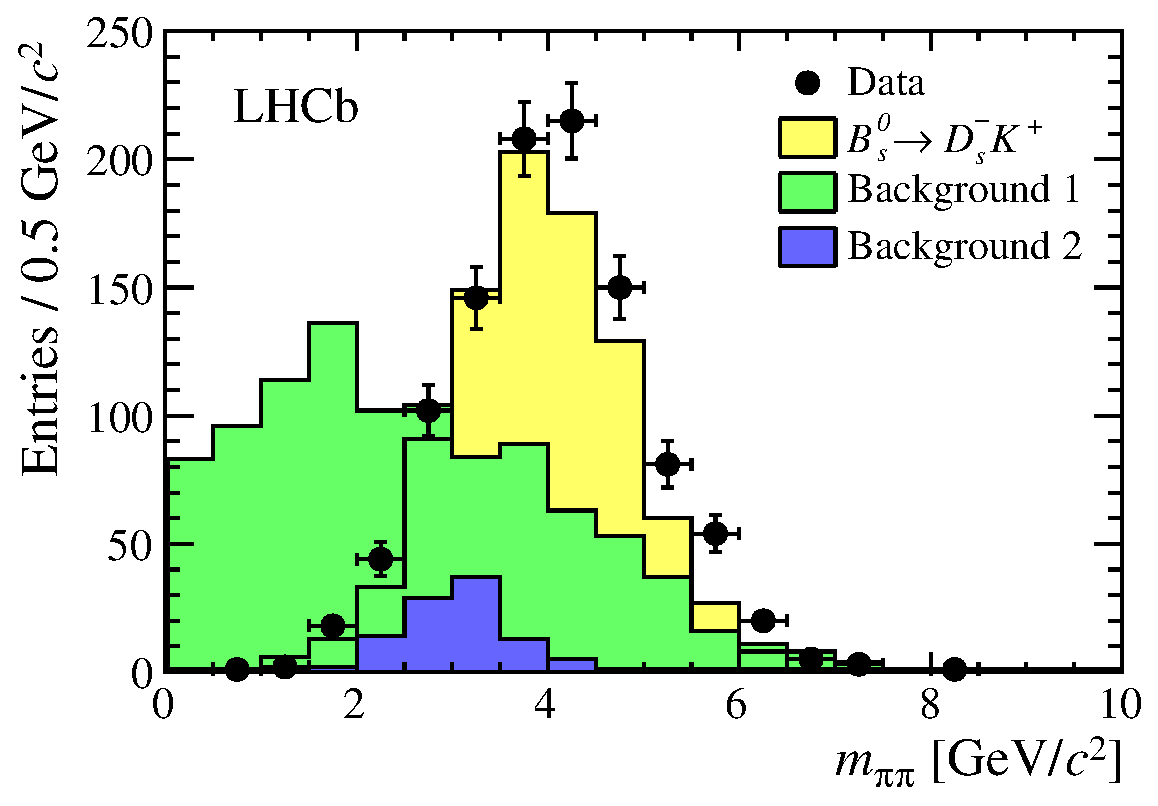
\includegraphics[width=0.7\linewidth]{Example1DPlot-python-1}
    \vspace*{-1.0cm}
  \end{center}
  \caption{
    \small %captions should be a little bit smaller than main text
    An example plot using the \lhcb style from the \erasmus package
    \texttt{RootTools/LHCbStyle}. The signal data is shown as points
    with the signal component as yellow (light), background 1 as green
    (medium) and background 2 as blue (dark).}
  \label{fig:example}
\end{figure}

\begin{enumerate}

\item Figures should be legible at the size they will appear in the
  publication, with suitable line width.  Their axes should be
  labelled, and have suitable units (e.g. avoid a mass plot with
  labels in MeV$/c^2$ if the region of interest covers a few GeV$/c^2$
  and all the numbers then run together).  Spurious background shading
  and boxes around text should be avoided.

\item Colour may be used in figures, but the distinction between
  differently coloured areas or lines should be clear also when the
  document is printed in black and white, for example through
  differently dashed lines. The \lhcb style mentioned above implements
  a colour scheme that works well but individual adjustments might be
  required.

\item Figures with more than one part should have the parts labelled
  (a), (b) etc., with a corresponding description in the caption;
  alternatively they should be clearly referred to by their position,
  e.g. Fig.~1\,(left).

\item All figures containing \lhcb data should have \lhcb written on
  them, preferably in the upper right corner.  For preliminary
  results, that should be replaced by ``LHCb preliminary''.

\end{enumerate}


\section{References}
\label{sec:References}

References should be made using Bib\TeX~\cite{BibTeX}. A special style
\texttt{LHCb.bst} has been created to achieve a uniform
style. Independent of the journal the paper is submitted to, the
preprint should be created using this style. Where arXiv numbers
exist, these should be added even for published articles. In the PDF
file, hyperlinks will be created to both the arXiv and the published
version.

\begin{enumerate}

\item Citations are marked using square brackets, and the
  corresponding references should be typeset using Bib\TeX\ and the
  official \lhcb Bib\TeX\ style. An example is in
  Ref.~\cite{Sjostrand:2006za}.

\item For references with four or less authors all of the authors'
  names are listed~\cite{Majorana:1937vz}, otherwise the first author
  is given, followed by \etal. the \lhcb Bib\TeX\ style will
  take care of this.

\item The order of references should be sequential when reading the
  document.

\item The titles of papers should in general be included. To remove
  them, change \texttt{\textbackslash
    setboolean\{articletitles\}\{false\}} to \texttt{true} at the top
  of this template.

\item The obtain the correct bibliographic information, the best
  option is to copy the Bib\TeX\ entry directly from
  \texttt{Inspire}. Some manual editing of the paper titles might be
  required to achieve correct \LaTeX\ formatting.

\item Even if the basic formatting of the Bib\TeX\ entry is taken from
  \texttt{Inspire}, all the data should be cross checked against the
  journal. Often there are minor changes to author initials or
  titles. In case of a difference between the preprint and the
  journal, the bibliographic information from the journal should be
  used.

\item The \texttt{mciteplus}~\cite{mciteplus} package is used in order
  to enable multiple references to show up as a single item in the
  reference list. As an example \texttt{\textbackslash
    cite\{Aaij:2011rj,*Pascoli:2007qh\}} where the \texttt{*}
  indicates that the reference should be merged with the previous
  one. The result of this can be seen in
  Ref.~\cite{Aaij:2011rj,*Pascoli:2007qh}. Be aware that the
  \texttt{mciteplus} package should be included as the very last item
  before the \texttt{\textbackslash begin\{document\}} to work
  correctly.

\item It should be avoided to make references to public notes and
  conference reports in public documents. Exceptions can be discussed
  on a case-by-case basis with the review committee for the
  analysis. In internal reports they are of course welcome and can be
  referenced as seen in~\cite{LHCb-CONF-2011-003} using the
  \texttt{lhcbreport} category. For conference reports, omit the
  author field completely in the Bib\TeX\ record.

\item To get the typesetting and hyperlinks correct for \lhcb reports,
  the category \texttt{lhcbreport} should be used in the Bib\TeX\
  file. See Ref.~\cite{LHCb-INT-2011-047, *LHCb-ANA-2011-078} for some
  examples. It can be used for \lhcb documents in the series
  \texttt{CONF}, \texttt{PAPER}, \texttt{PROC}, \texttt{THESIS}, and
  internal \lhcb reports. Papers sent for publication, but not
  published yet, should be referred with their \texttt{arXiv} number,
  so the \texttt{PAPER} category should only be used in the rare case
  of a forward reference to a paper.

\item Proceedings can be used for references to items such as the
  \lhcb simulation~\cite{LHCb-PROC-2011-006}, where we do not yet have
  a published paper.

\end{enumerate}

There is a set of standard references to be used in \lhcb that are
listed in Appendix~\ref{sec:StandardReferences}.


\section{Inclusion of supplementary material}
\label{sec:Supplementary}

In some cases it is desirable to approve material that is
supplementary to that which is included in the main body of the paper.
For example, sometimes a short letter paper is written, but additional
figures that cannot be contained within the page limit should be
approved to be available to be shown in talks. As a reminder, only
approved material can be shown in public. Another use case is to
provide data tables.  Any supplementary material should be made
available in the circulation to the collaboration in a clearly marked
appendix to the main document.  Before the paper is submitted this
appendix must be removed, and the supplementary material is added
separately to the CDS entry.

Journals published through or by the AIP, such as Phys. Rev. Lett. and
Phys. Rev. D, support the use of
\href{http://www.aip.org/pubservs/epaps.html}{EPAPS}.  Their
description of relevant supplementary material includes
\begin{quote} {\it multimedia (e.g., movie files, audio files,
    animated .gifs, 3D rendering files), color figures, data tables,
    and text (e.g., appendices) that are too lengthy or of too limited
    interest for inclusion in the printed journal}.
\end{quote}
LHCb publications in those journals can make of EPAPS as appropriate.
However, note that there are some categories of supplementary
material, such as additional plots, that are not appropriate for
EPAPS.

The appendix containing supplementary material should not normally be
referred to in the main body of the text as it will not appear in
the final version.  An exception is for material that will be
available in EPAPS, where the
\href{http://www.aip.org/epaps/how_epaps_works.html#deposit}{AIP
  recommendation} is
\begin{quote} {\it Files are made available to users via links from
    the journal. Authors should include a reference in the form ``See
    supplementary material at [URL will be inserted by AIP] for [give
    brief description of material].''}
\end{quote}
However, in this template, an example of the formatting for an appendix
of supplementary material is given in
Appendix~\ref{sec:Supplementary-App}.


% Do not include this in analysis note and conference reports
\section*{Acknowledgements}

\noindent We express our gratitude to our colleagues in the CERN
accelerator departments for the excellent performance of the LHC. We
thank the technical and administrative staff at the LHCb
institutes. We acknowledge support from CERN and from the national
agencies: CAPES, CNPq, FAPERJ and FINEP (Brazil); NSFC (China);
CNRS/IN2P3 and Region Auvergne (France); BMBF, DFG, HGF and MPG
(Germany); SFI (Ireland); INFN (Italy); FOM and NWO (The Netherlands);
SCSR (Poland); ANCS/IFA (Romania); MinES, Rosatom, RFBR and NRC
``Kurchatov Institute'' (Russia); MinECo, XuntaGal and GENCAT (Spain);
SNSF and SER (Switzerland); NAS Ukraine (Ukraine); STFC (United
Kingdom); NSF (USA). We also acknowledge the support received from the
ERC under FP7. The Tier1 computing centres are supported by IN2P3
(France), KIT and BMBF (Germany), INFN (Italy), NWO and SURF (The
Netherlands), PIC (Spain), GridPP (United Kingdom). We are thankful
for the computing resources put at our disposal by Yandex LLC
(Russia), as well as to the communities behind the multiple open
source software packages that we depend on.


% $Id: appendix.tex 30551 2013-01-25 19:09:21Z uegede $
% ===============================================================================
% Purpose: appendix to the standard template: standard symbol alises from Ulrik
% Author: Tomasz Skwarnicki
% Created on: 2009-09-24
% ===============================================================================

\clearpage

{\noindent\bf\Large Appendix}

\appendix

\section{List of Required Jenkins Plug-Ins}
\label{sec:JenkinsPlugIns}
Here is summarized the list of plug-ins that are required to configure Jenkins
to run the nightly builds
\newcommand{\JPI}[2]{\item \link{#2}{#1}}
\begin{itemize}
  \JPI{Build Name Setter Plugin}%
  {http://wiki.jenkins-ci.org/display/JENKINS/Build+Name+Setter+Plugin}
  \JPI{Copy Artifact Plugin}%
  {http://wiki.jenkins-ci.org/display/JENKINS/Copy+Artifact+Plugin}
  \JPI{Dynamic Axis Plugin}%
  {http://wiki.jenkins-ci.org/display/JENKINS/DynamicAxis+Plugin}
  \JPI{Groovy Plugin}%
  {http://wiki.jenkins-ci.org/display/JENKINS/Groovy+plugin}
  \JPI{Jenkins GIT Plugin}%
  {http://wiki.jenkins-ci.org/display/JENKINS/Git+Plugin}
  \JPI{Jenkins Parameterized Trigger Plugin}%
  {http://wiki.jenkins-ci.org/display/JENKINS/Parameterized+Trigger+Plugin}
  \JPI{Jenkins SSH Slaves Plugin}%
  {http://wiki.jenkins-ci.org/display/JENKINS/SSH+Slaves+plugin}
  \JPI{Jenkins Workspace Cleanup Plugin}%
  {http://wiki.jenkins-ci.org/display/JENKINS/Workspace+Cleanup+Plugin}
  \JPI{Matrix Tie Parent Plugin}%
  {http://wiki.hudson-ci.org/display/HUDSON/Matrix+Tie+Parent+Plugin}
  \JPI{Node and Label Parameter Plugin}%
  {http://wiki.jenkins-ci.org/display/JENKINS/NodeLabel+Parameter+Plugin}
\end{itemize}

The following list contains the plug-ins not needed for the jobs configuration,
but useful for management tasks
\begin{itemize}
  \JPI{Bulk
Builder}{http://wiki.jenkins-ci.org/display/JENKINS/Bulk+Builder+Plugin}
  \JPI{Jenkins Disk Usage
Plugin}{http://wiki.jenkins-ci.org/display/JENKINS/Disk+Usage+Plugin}
  \JPI{Rebuilder}{http://wiki.jenkins-ci.org/display/JENKINS/Rebuild+Plugin}
  \JPI{Recipe Plugin}{https://wiki.jenkins-ci.org/display/JENKINS/Recipe+Plugin}
  \JPI{Shelve Project
Plugin}{http://wiki.jenkins-ci.org/display/JENKINS/Shelve+Project+Plugin}
\end{itemize}

% \section{To-Do List}
% \begin{itemize}
%   \item Configuration
%   \begin{itemize}
%     \item allow inclusion of shared configuration files (e.g. for the
% environment)
%     \item use the environment settings in all the steps
%     \item review the \emph{plug-in} mechanism
%     \item define where to store the configuration of the slots
%   \end{itemize}
%   \item Build
%   \begin{itemize}
%     \item check if the build produced files in the source directories
%   \end{itemize}
%   \item Tests
%   \begin{itemize}
%     \item integration between QMTest and CTest
%   \end{itemize}
%   \item Dashboard
%   \item Jenkins
%   \begin{itemize}
%     \item simplified node labels and matching (e.g. x86\_64-slc5-gcc46-dbg
% $\rightarrow$ slc5)
%   \end{itemize}
%
% \end{itemize}


% This should be taken out in the final paper
\clearpage

\section{Supplementary Material}
\label{sec:Supplementary-App}

{\bf This appendix includes supplementary material that will be made
  available on CDS during the review phase but will not appear in the
  final version of the paper.}

\begin{figure}[!htb]
  \begin{center}
    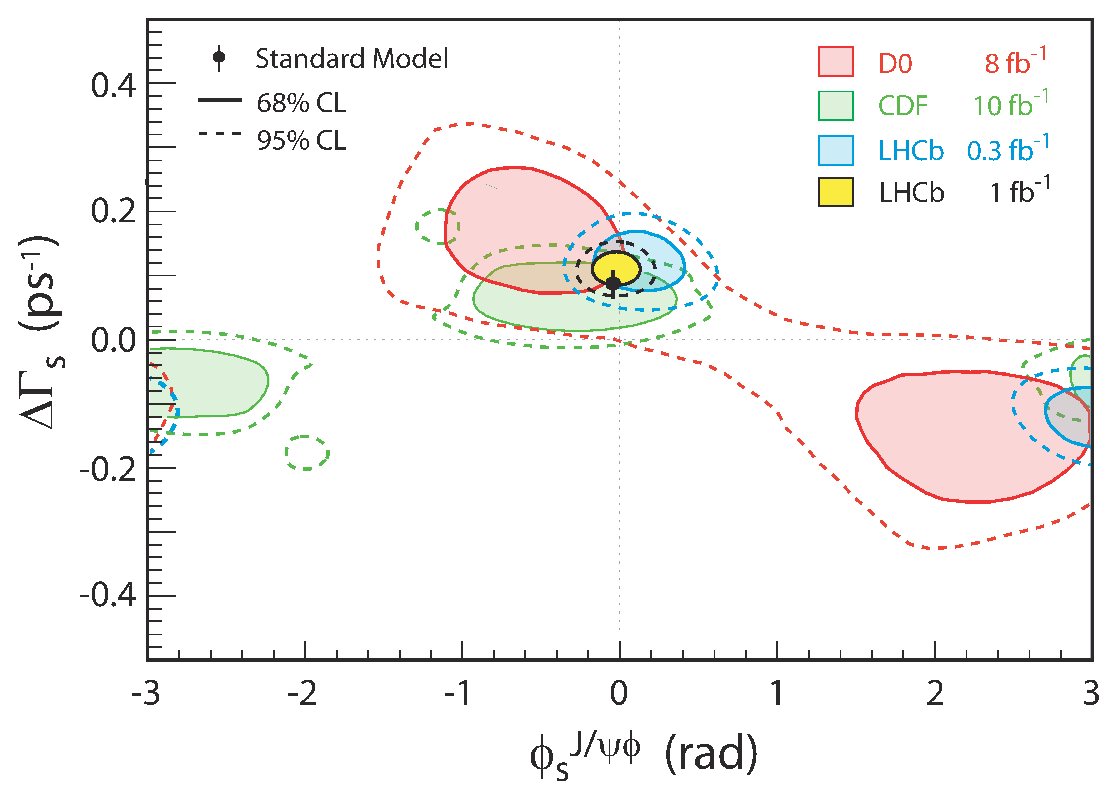
\includegraphics[scale=0.65,bb=50 300 580 700,clip=true]{Roger-plot}
    \vspace*{-1.0cm}
  \end{center}
  \caption{
    \small %captions should be a little bit smaller than main text
    This plot compares our result to those from other experiments.}
  \label{fig:roger}
\end{figure}

\clearpage



\addcontentsline{toc}{section}{References}
\bibliographystyle{LHCb}
\bibliography{main,LHCb-PAPER,LHCb-CONF}

\end{document}
